\documentclass[11pt, twoside, pdftex]{article}

% This includes all the settings that we should use for the document
\newcommand{\PDFTitle}{\productNameMed{} Tutorial}
\newcommand{\commonPath}{../../Common}
\newcommand{\datePublished}{Mar 2022}

\newcommand{\versnum}{21.1} %version number quartus/AMP
\newcommand{\quartusname}{Quartus\textsuperscript{\textregistered} Prime}	
\newcommand{\textBar}{For \quartusname{} \versnum{}}
\newcommand{\thisyear}{2022 } %for copyright
\newcommand{\company}{FPGAcademy.org}
\newcommand{\longteamname}{FPGAcademy.org}
\newcommand{\teamname}{FPGAcademy}
\newcommand{\website}{FPGAcademy.org}

\newcommand{\productAcronym}{AMP}
\newcommand{\productNameShort}{Monitor Program}

\newcommand{\productNameMedTM}{Monitor Program}
\newcommand{\productNameMed}{Monitor Program}

%\newcommand{\headerLogoFilePath}[1]{#1/FPGAcademy.png}



\setlength\topmargin{-0.25in}
\setlength\headheight{0in}
\setlength\headsep{0.35in}
\setlength\textheight{8.5in}
\setlength\textwidth{7in}
\setlength\oddsidemargin{-0.25in}
\setlength\evensidemargin{-0.25in}
\setlength\parindent{0.25in}
\setlength\parskip{0in} 

\pdfpagewidth 8.5in
\pdfpageheight 11in

% listings is a package that supports encapsulating source code in LaTeX conveniently

\usepackage{listings}
% add support for graphics
\usepackage{graphicx}
\usepackage[usenames, dvipsnames]{color}

\def\expandparam\lstinputlisting[#1]#2{\edef\tmp{\noexpand\lstinputlisting[#1]{#2}}\tmp}

\widowpenalty 10000
\clubpenalty 10000

%%%%%%%%%%%%%%%%%%%% Source Code Formatting %%%%%%%%%%%%%%%%%%%%
\definecolor{globalCommentColour}{rgb}{0.588,0.588,0.588}

%%%%%%%%%%%%%%%%%%%%%%%%%%%%%%%%%%%%%%%%%%%%%%%%%%%%
% Defining a NiosII ASM highlighter for lstlisting
\lstdefinelanguage[NiosII]{Assembler} {
 	morekeywords={add, addi, and, andhi, andi, beq, bge, bgeu, bgt, bgtu, ble,  bleu, blt, bltu, bne, br, break,% 
 	bret, call, callr, cmpeq, cmpeqi, cmpge, cmpgei, cmpgeu, cmpgeui, cmpgt, cmpgti, cmpgtu, cmpgtui, cmple,%
 	cmplei, cmpleu, cmpleui, cmplt, cmplti, cmpltu, cmpltui, cmpne, cmpnei, custom, div, divu, eret, flushd,%
 	flushda, flushi, flushp, initd, initda, initi, jmp, jmpi, ldb, ldbio, ldbu, ldbuio, ldh, ldhio, ldhu, ldhuio,%
 	ldw, ldwio, mov, movhi, movi, movia, movui, mul, muli, mulxss, mulxsu, mulxuu, nextpc, nop, nor, or, orhi, ori,%
 	rdctl, rdprs, ret, rol, roli, ror, sll, slli, sra, srai, srl, srli, stb, stbio, sth, sthio, stw, stwio,%
 	sub, subi, sync, trap, wrctl, wrtcl, wrprs, xor, xori, xorhi, xori},% 	
 	morekeywords=[2]{.abort, .ABORT, .align, .app-file, .ascii, .asciz, .balign, .byte, .comm, .data, .def,%
 	.desc, .dim, .double, .eject, .else, .end, .endef, .endif, .equ, .equiv, .err, .extern, .file, .fill, .float,%
 	.global, .globl, .hword, .ident, .if, .include, .int, .irp, .irpc, .lcomm, .lflags, .line, .linkonce, .ln,%
 	.list, .long, .macro, .mri, .nolist, .octa, .org, .p2align, .psize, .quad, .rept, .sbttl, .scl, .section,%
 	.set, .short, .single, .size, .sleb128, .skip, .space, .stadb, .stabn, .stabs, .string, .symver, .tag,%
 	.text, .title, .type, .val, .uleb128, .word},% 	
 	morekeywords=[3]{et, bt, gp, sp, fp, ea, sstatus, ra, pc, status, estatus, bstatus, ienable, ipending, cpuid,%
 	exception, pteaddr, tlbacc, tlbmisc, eccinj, badaddr, config, mpubase, mpuacc},% 	
 	sensitive=t,%
 	alsoletter=.,%
	morestring=[b]",%
 	morecomment=[s]{/*}{*/},%
 	morecomment=[l]\#,%
   }[keywords,comments,strings]
   
   %% NOTE: morekeywords=[2] are GNU directives.
   
   \definecolor{niosInstructionColour}{rgb}{0.000,0.608,0.000}
   \definecolor{niosDirectiveColour}{rgb}{0.000,0.000,0.902}
   \definecolor{niosSpecialRegColour}{rgb}{0.000,0.000,0.000}
   \definecolor{niosStringColour}{rgb}{0.808,0.482,0.000}
   
   %% NOTE: To make bold use: =\bfseries\color{<colour>}
   \lstdefinestyle{defaultNiosStyle} {
   language=[NiosII]{Assembler},
   stringstyle=\color{niosStringColour},
   keywordstyle=\color{niosInstructionColour},
   keywordstyle=[2]\color{niosDirectiveColour},
   keywordstyle=[3]\itshape\color{niosSpecialRegColour}
   }
%%%%%%%%%%%%%%%%%%%%%%%%%%%%%%%%%%%%%%%%%%%%%%%%%%%%

%%%%%%%%%%%%%%%%%%%%%%%%%%%%%%%%%%%%%%%%%%%%%%%%%%%%
% Defining a ArmA9 ASM highlighter for lstlisting
\lstdefinelanguage[ArmA9]{Assembler} {
 	morekeywords={ADC, ADD, ADDS, AND, ANDS, B, BAL, BEQ, BGE, BGT, BL, BLT, BIC, BKPT, BLX, BNE, BX, CDP, CLZ, CMN, CMP, EOR,%
 	EORS, LDC, LDM, LDR, LDRB, LDRBT, LDRH, LDRSB, LDRSH, LDRT, LSL, MCR, MLA, MOV, MOVW, MOVT, MRC, MRS, MSR, MUL, MVN, ORR, PLD,%
 	ROR, RSB, RSC, SBC, SMLAL, SMULL, STC, STM, STR, STRB, STRBT, STRH, STRT, SUB, SUBS, SWI, SWP, SWPB, TEQ, UMLAL,
 	PUSH, POP, MOVS, RORS, LSR},%
 	morekeywords=[2]{.abort, .ABORT, .align, .app-file, .ascii, .asciz, .balign, .byte, .comm, .data, .def,%
 	.desc, .dim, .double, .eject, .else, .end, .endef, .endif, .equ, .equiv, .err, .extern, .file, .fill, .float,%
 	.global, .globl, .hword, .ident, .if, .include, .int, .irp, .irpc, .lcomm, .lflags, .line, .linkonce, .ln,%
 	.list, .long, .macro, .mri, .nolist, .octa, .org, .p2align, .psize, .quad, .rept, .sbttl, .scl, .section,%
 	.set, .short, .single, .size, .sleb128, .skip, .space, .stadb, .stabn, .stabs, .string, .symver, .tag,%
 	.text, .title, .type, .val, .vectors, .uleb128, .word},%
 	morekeywords=[3]{SP, PC, MIDR, CTR, TCMTR, TLBTR, MPIDR, ID_PFR0, ID_PFR1, ID_DFR0, ID_MMFR0, ID_MMFR1, ID_MMFR2,%
 	ID_MMFR3, ID_ISAR0, ID_ISAR1, ID_ISAR2, ID_ISAR3, ID_ISAR4, CCSIDR, CLIDR, AIDR, CSSELR, TTBR0, TTRB1, TTBR2, DACR,%
 	DFSR, IFSR, ADFSR, AIFSR, DFAAR, IFAR, ICIALLUIS, BPIALLIS, PAR, ICIALLU, ICIMVAU, BPIALL, DCIMVAC, DCISW, V2PCWPR,%
 	DCCVAC, DCCSW, DDIMVAC, DCISW, TLBALLIS, TLBIMVAIS, TLBIASIDIS, TLBIMVAAIS, TLBIALL, TLBIMVA, TLBIASID, TLBIMVAA,%
 	PMCR, PMCNTENSET, PMCNTENCLR, PMOVSR, PMSWINC, PMSELR, PMXEVTYPER, PMXEVCNTR, PMUSERENR, PMINTENSET, PMINTENCLR,%
 	PRRR, NRRR, PLEIDR, PLEASR, PLEFSR, PLEUAR, PLEPCR, VBAR, MVBAR, ISR, FCSEIDR, CONTEXTIDR, TPIDRURW, TPIDRURO, TPIDRPRW},%
 	sensitive=f,%
 	alsoletter=.,%
	morestring=[b]",%
 	morecomment=[s]{/*}{*/},%
 	morecomment=[l]{//},%
   }[keywords,comments,strings]
   
   %% NOTE: morekeywords=[2] are GNU directives.
   
   \definecolor{armInstructionColour}{rgb}{0.000,0.608,0.000}
   \definecolor{armDirectiveColour}{rgb}{0.000,0.000,0.902}
   \definecolor{armSpecialRegColour}{rgb}{0.000,0.000,0.000}
   \definecolor{armStringColour}{rgb}{0.808,0.482,0.000}
   
   \lstdefinestyle{defaultArmStyle} {
   language=[ArmA9]{Assembler},
   stringstyle=\color{armStringColour},
   keywordstyle=\color{armInstructionColour},
   keywordstyle=[2]\color{armDirectiveColour},
   keywordstyle=[3]\itshape\color{armSpecialRegColour}
   }
%%%%%%%%%%%%%%%%%%%%%%%%%%%%%%%%%%%%%%%%%%%%%%%%%%%%

%%%%%%%%%%%%%%%%%%%%%%%%%%%%%%%%%%%%%%%%%%%%%%%%%%%%
% Defining style for the verilog.

\definecolor{verilogCommentColour}{rgb}{0.000,0.502,0.000}

\lstdefinestyle{defaultVerilogStyle} {
language={Verilog},
keywordstyle=\color{blue},
commentstyle=\color{verilogCommentColour}
}
%%%%%%%%%%%%%%%%%%%%%%%%%%%%%%%%%%%%%%%%%%%%%%%%%%%%

%%%%%%%%%%%%%%%%%%%%%%%%%%%%%%%%%%%%%%%%%%%%%%%%%%%%
% Defining style for the vhdl.
\lstdefinestyle{defaultVHDLStyle} {
language={VHDL},
keywordstyle=\color{blue},
commentstyle=\color{verilogCommentColour}
}
%%%%%%%%%%%%%%%%%%%%%%%%%%%%%%%%%%%%%%%%%%%%%%%%%%%%

%%%%%%%%%%%%%%%%%%%%%%%%%%%%%%%%%%%%%%%%%%%%%%%%%%%%
% Java
\definecolor{javaStringColour}{rgb}{0.808,0.482,0}
%%%%%%%%%%%%%%%%%%%%%%%%%%%%%%%%%%%%%%%%%%%%%%%%%%%%

%%%%%%%%%%%%%%%%%%%%%%%%%%%%%%%%%%%%%%%%%%%%%%%%%%%%
% Defining language styles
% C
\definecolor{CStringColour}{rgb}{0.808,0.482,0}
%%%%%%%%%%%%%%%%%%%%%%%%%%%%%%%%%%%%%%%%%%%%%%%%%%%%

%%%%%%%%%%%%%%%%%%%%%%%%%%%%%%%%%%%%%%%%%%%%%%%%%%%%
% Defining extended LaTeX language.
\lstdefinelanguage[LocalLaTeX]{TeX}[LaTeX]{TeX}%
 	{moretexcs={bf, it, sf, lstset},%
   	}%

\lstdefinestyle{defaultLocalLatexStyle} {
language=[LocalLatex]{TeX},
keywordstyle=\color{blue}\bfseries,
keywordstyle=[2]\color{blue},
keywordstyle=[3]\color{blue}\bfseries
}
%%%%%%%%%%%%%%%%%%%%%%%%%%%%%%%%%%%%%%%%%%%%%%%%%%%%

\lstset{
%language = C,
%language = Verilog,
%basicstyle=\color{black}\rmfamily\ttfamily,
basicstyle=\small\color{black}\ttfamily,
commentstyle=\small\color{globalCommentColour}\itshape\ttfamily,
keywordstyle=\small\color{blue}\bfseries\ttfamily,
showstringspaces=false,
frame=none, %lines % boxed listings
breaklines=true,
breakatwhitespace=true,
tabsize=4
}
%%%%%%%%%%%%%%%%%%%%%%%%%%%%%%%%%%%%%%%%%%%%%%%%%%%%%%%%%%%%%%%%


%\usepackage[centering]{geometry}.
%%%%%%%%%%%%%%%%%%%%%%%%%%%%%%%%%%%%%%%%%%%%%%%%%%%
% Document Settings
\usepackage[labelsep=period]{caption}
% we can choose a better font later
%\usepackage{palatino}
\usepackage{fourier}
%\fontencoding{T1}
% include common used symbols
\usepackage{textcomp}
% add support for graphics
\usepackage{graphicx}
\usepackage[usenames, dvipsnames]{color}
% enable to draw thick or thin table hlines
\setlength{\doublerulesep}{\arrayrulewidth}
\usepackage{longtable}
\setlongtables
%\usepackage{array}
% It may be better to use PDFLaTeX as it can generate bookmarks for the
% document

% Add some useful packages
\usepackage{ae,aecompl}
\usepackage{epsfig,float,times}

% reset the font for section
\usepackage{sectsty}
%\allsectionsfont{\fontfamily{ptm}\selectfont}
\allsectionsfont{\usefont{OT1}{phv}{bc}{n}\selectfont}

% use compact space for sections
\usepackage[compact]{titlesec}
\titlespacing{\section}{0pt}{0.2in}{*0}
\titlespacing{\subsection}{0pt}{0.1in}{*0}
\titlespacing{\subsubsection}{0pt}{0.05in}{*0}

% fancyhdr header and footer customization
\usepackage{layout}
\usepackage{fancyhdr}
\pagestyle{fancy}
\fancyhead{}
\fancyhead[R]{\textit{\tiny{\textBar}}}
\fancyfoot{}
\fancyfoot[LO,
RE]{\textrm{\href{https://www.fpgacademy.org}{\small \longteamname}} \\ {\small \datePublished }}
\fancyfoot[RO, LE]{\small \thepage}
% two-side settings
%\fancyhead{} % clear all header fields
%\fancyfoot{} % clear all footer fields
%\fancyfoot[LE,RO]{\thepage}
\renewcommand{\headrulewidth}{2pt}
\renewcommand{\headrule}{{\color{blue} \hrule width\headwidth height\headrulewidth \vskip-\headrulewidth}}
\renewcommand{\footrulewidth}{0pt}

% Format the footer on page 1
\fancypagestyle{plain}{
\fancyhead{}
\fancyfoot{}
\fancyfoot[LO,
RE]{\textrm{\href{https://www.fpgacademy.org}{\small \longteamname}} \\ {\small \datePublished }}
\fancyfoot[RO, LE]{\small \thepage}
\renewcommand{\headrulewidth}{0pt}
}
% adjust some setting to try to make the figure stay in the same page with text
% Reference: 	http://www.cs.uu.nl/~piet/floats/node1.html
%   			http://mintaka.sdsu.edu/GF/bibliog/latex/floats.html
%   General parameters, for ALL pages:
\renewcommand{\topfraction}{0.9}	% max fraction of floats at top
\renewcommand{\bottomfraction}{0.8}	% max fraction of floats at bottom
%   Parameters for TEXT pages (not float pages):
\setcounter{topnumber}{3}
\setcounter{bottomnumber}{3}
\setcounter{totalnumber}{5}     % 2 may work better
\setcounter{dbltopnumber}{2}    % for 2-column pages
\renewcommand{\dbltopfraction}{0.9}	% fit big float above 2-col. text
\renewcommand{\textfraction}{0.07}	% allow minimal text w. figs
%   Parameters for FLOAT pages (not text pages):
\renewcommand{\floatpagefraction}{0.7}	% require fuller float pages
% N.B.: floatpagefraction MUST be less than topfraction !!
\renewcommand{\dblfloatpagefraction}{0.7}	% require fuller float pages
%%%%%%%%%%%%%%%%%%%%%%%%%%%%%%%%%%%%%%%%%%%%%%%%%%%
% remember to use [htp] or [htpb] for placement
%%%%%%%%%%%%%%%%%%%%%%%%%%%%%%%%%%%%%%%%%%%%%%%%%%%

% set no indent for paragraph
\setlength{\parindent}{0em}
\addtolength{\parskip}{11pt}
\newcommand{\compact}{[topsep=0pt]}
% use this package to reduce space
\usepackage{enumitem}
\usepackage{multirow}
\usepackage{rotating}
\usepackage{pifont}
\usepackage{dingbat}
\newcommand{\itemsecond}{$\circ$}
%
%%%%%%%%%%%%%%%%%%
\date{}
\author{}
%%%%%%%%%%%%%%%%%%
\newcommand{\de}{DE-series}
\newcommand{\up}{FPGAcademy}
\newcommand{\fabric}{Avalon Switch Fabric}
\newcommand{\TODO}[1]{\textcolor{red}{\textbf{TODO}: #1}}
\def\registered{{\ooalign{\hfil\raise .00ex\hbox{\scriptsize R}\hfil\crcr\mathhexbox20D}}}

% enable url and reference(bookmarks) in pdf
\usepackage{url}
\usepackage[pdftex, colorlinks]{hyperref}
\hypersetup{%
pdftitle={\PDFTitle},
linkcolor=blue,
hyperindex=true,
pdfauthor={\longteamname},
pdfkeywords={FPGAcademy, Academic Program, Example System},
bookmarksnumbered,
bookmarksopen=false,
filecolor=blue,
pdfstartview={FitH},
urlcolor=blue,
plainpages=false,
pdfpagelabels=true,
linkbordercolor={1 1 1} %no color for link border
}%
%%%%%%%%%%%%%%%%%%%%%%%%%%%%%%%%%%%%%%%%%%%%%%%%%%%
\setlength{\fboxsep}{0.7pt}
\setlength{\fboxrule}{0.5pt}

\newcommand{\red}[1]{{\color{red}\sf{#1}}}
\newcommand{\blue}[1]{{\color{blue}\sf{#1}}}



%%%%%%%%%%%%%%%%%%%%%%%%%
% Add title
\newcommand{\doctitle}{\productNameMed{} Manual}
\newcommand{\dochead}{\productNameMed{} Manual}
% Usually no need to change these two lines
\title{\fontfamily{phv}\selectfont{\doctitle} }
\chead{ \small{\textsc{\bfseries \dochead} } }
% Customizations
\usepackage{hyperref}
%%%%%%%%%%%%%%%%%%%%%%%%%
% Allows multiple figures per page

\renewcommand\floatpagefraction{.9}
\renewcommand\topfraction{.9}
\renewcommand\bottomfraction{.9}
\renewcommand\textfraction{.1}   
\setcounter{totalnumber}{50}
\setcounter{topnumber}{50}
\setcounter{bottomnumber}{50}
\widowpenalty 10000
\clubpenalty 10000
\raggedbottom

%%%%%%%%%%%%%%%%%%
%%% DOCUMENT START
%\begin{document}
\begin{document}
\begin{table}
    \centering
    \begin{tabular}{p{5cm}p{4cm}}
        \hspace{-3cm}
        &
        \raisebox{1\height}{\parbox[h]{0.5\textwidth}{\Large\fontfamily{phv}\selectfont{\textsf{\doctitle}}}}
    \end{tabular}
    \label{tab:logo}
\end{table}

\colorbox[rgb]{0,0.384,0.816}{\parbox[h]{\textwidth}{\color{white}\textsf{\textit{\textBar}}}}

\thispagestyle{plain}
 
\section{Introduction}

This is a user manual for the \productNameMed{}, which can
be used to compile, assemble, download and debug programs for
either Intel's Nios~II processor or for ARM processor. 
The manual is intended for a user who wishes to use either
Nios II or ARM based systems on an Intel Development and
Education board. Features of the Monitor Program are detailed 
through a combination of step-by-step tutorials (for both ARM and Nios II) and descriptions.
You do not need to follow the tutorial from beginning to end to learn
about the features of the Monitor Program, but if you wish to do so
you may follow the italicized tutorial hyperlinks to sequentially view
all tutorial sections.

{\it To start going through the tutorials in this document, click \hyperref[tut:start]{here}.}

The Monitor Program is a software application which runs on a
host PC, and communicates with either a Nios~II based or an ARM
based hardware system implemented on an FPGA board. It can be
used to compile/assemble a user program, download the
program onto the FPGA board, and then debug the running
program. It provides features that allow a user to:

\begin{itemize}
    \item Set up a project that specifies a desired
hardware system and software program
    \item Download the hardware system onto an FPGA board
    \item Compile software programs, specified in assembly language or C language , and download the resulting machine code
into the hardware system
    \item Display the generated machine code stored in memory
    \item Run the processor, either continuously or by single-stepping instructions
    \item Examine and modify the contents of processor registers
    \item Examine and modify the contents of memory, as well as
memory-mapped registers in I/O devices
    \item Set breakpoints that stop the execution of a program at
a specified address, or when certain conditions are met
    \item Develop programs that make use of device driver functions provided through Intel's Hardware Abstraction Layer
(HAL)
\end{itemize}

The process of downloading and debugging an application program
requires an FPGA board to implement the desired hardware system.
In this document it is assumed that the reader has access to the
Intel DE1-SoC Development and Educaton board, connected to a
computer that has Quartus Prime 
and Nios~II Embedded Design Suite (EDS) software installed. 

\subsection{Who should use the Monitor Program}

The Monitor Program is intended to be used in an educational
environment by professors and students. It is not intended for
commercial use.

\section{Installing the Monitor Program}

The Monitor Program is released as part of Intel's FPGA University
Program Design Suite (UPDS). Before the UPDS can be installed on
a computer, it is necessary to first install Intel's Quartus Prime
CAD software (either the Web Edition or Subscription Edition) 
and the Nios~II Embedded Design Suite (EDS). A particular release
of the Monitor Program can be used only with a corresponding version of the Quartus~Prime software and Nios~II EDS. This software
can be obtained from the {\it Download Center} on Intel's
website at {\it www.altera.com}.
To locate the software select {\it DOWNLOADS} and then download
the desired version.

Once the Quartus Prime software and Nios~II EDS are installed,
the Intel UPDS can be installed.

Note that if the Quartus Prime software is re-installed at some
future time, then it will be necessary to re-install the Monitor
Program at that time.

\subsection{Using a Windows Operating System}

When using a Windows operating system, perform the following: 

\begin{enumerate}
\item Install the Intel UPDS from the University Program section of Intel's \href{https://www.intel.com/content/www/us/en/programmable/support/training/university/materials-software.html}{website}.
Specify the installed version of Quartus Prime software.
Then click on the {\it EXE} item in the displayed table, 
which links to an installation program called 
{\it intel\_fpga\_upds\_setup.exe}. When prompted to 
{\sf Run} or {\sf Save} this file, select {\sf Run}. 
		  
\item The first screen of the installer is shown in Figure \ref{fig:UPDS_setup_start}.
Click on the {\sf Next} button.

 \item The installer will display the License Agreement; if you accept the terms of this agreement, then click {\sf I Agree} to
continue.
	
\item The installer now displays the root directory where the
Intel FPGA University Program Design Suite will be installed.  
Click {\sf Next}.

\item The next screen, shown in Figure \ref{fig:UPDS_setup_installdir}, lists the components that will be installed, which include the Monitor Program
software and University Program IP Cores. These IP Cores provide
a number of I/O device circuits that can be used in hardware
systems to be implemented on the FPGA board.

\item The installer is now ready to begin copying files. 
Click {\sf Install} to proceed and then click {\sf Next} after
the installation has been completed. 
If you answered {\sf Yes} when prompted about placing a shortcut on your Windows Desktop, then an icon 
\hbox{
\includegraphics[scale=0.65]{images/img_shortcut_sm.png}}
is provided on the Desktop that can be used to start the Monitor
Program.

\begin{figure}[H]
	\begin{center}
		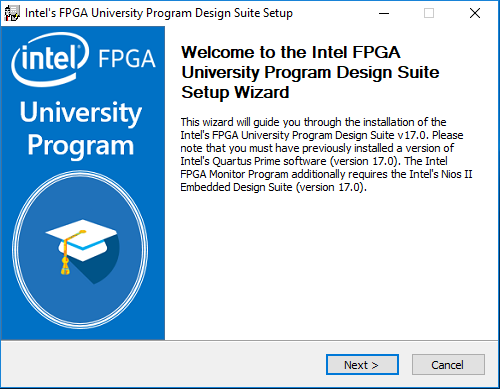
\includegraphics[scale=1]{screenshots/figure1.png}
	\end{center}
	\caption{Intel UPDS Setup Program.}
	\label{fig:UPDS_setup_start}
\end{figure}

\begin{figure}[H]
   	\begin{center}
            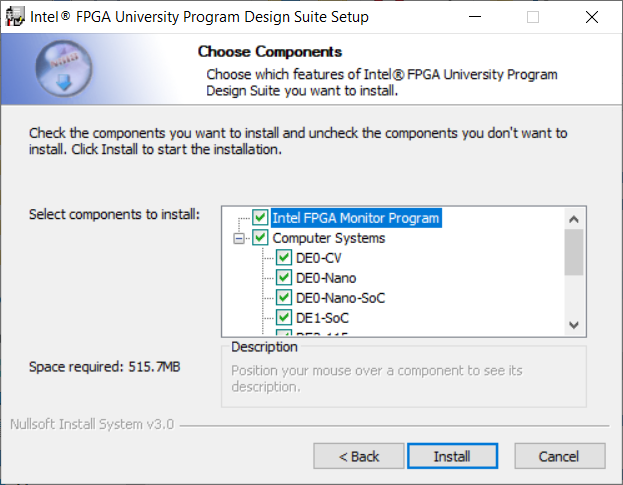
\includegraphics[scale=0.9]{screenshots/figure2.png}
   	\end{center}
      \caption{The components that will be installed.}
      \label{fig:UPDS_setup_installdir}
\end{figure}
~\\

\item Now, the Intel's FPGA University Program Design Suite is successfully installed on your computer; click {\sf Finish} to
finish the installation.

\item Should an error occur during the installation procedure, a pop-up window will suggest the appropriate action. 
Possible errors include:
\begin{itemize}
\item Quartus Prime software is not installed or the Quartus Prime
version is incorrect.
\item Nios~II EDS software is not installed or the version is
incorrect.
\end{itemize}
\end{enumerate}


\subsection{Using a Linux Operating System}

When using a Linux operating system, perform the following:

\begin{enumerate} 
\item Install the Intel UPDS from the University Program section of Intel's website. It can be found by going to {\it https://www.intel.com/content/www/us/en/programmable/support/training/university/materials-software.html}.
Specify the installed version of Quartus Prime software.
Then click on the {\it TAR} item in the displayed table, 
which links to an installation tarball called 
{\it intel\_fpga\_upds\_setup.tar}. 
Save this file to a directory of your choosing.

\item Using a console, navigate to the directory to which the
file was saved. Extract the contents of 
{\it intel\_fpga\_upds\_setup.tar} using the following command: 
{\bf tar -xf intel\_fpga\_upds\_setup.tar}.

\item Among the extracted files is a shell script named
{\it install\_intel\_fpga\_upds} which will be used to install the
UPDS. Ensure that the script is executable by using the following
command: {\bf chmod +x install\_intel\_fpga\_upds}. 

\item Run the installation script with superuser privileges by
using the following command: 
{\bf sudo ./install\_intel\_fpga\_upds}.

\item Follow the instructions displayed by the script to complete
the installation.

\end{enumerate}

\section{Creating a Project}
\label{tut:start}

Each software application that is developed with the
\productNameMed{} is called a {\it project}. 
The Monitor Program works on one project at a time and keeps all information for that project in a single directory in the file
system. The first step is to create a directory to hold the project's files. To store the design files for this document, 
we will use a directory named {\it Monitor\_Manual}. 
As a running example we will use a simple assembly-language
program that controls some lights on a DE1-SoC board.

If you are using a Windows operating system, then
start the Monitor Program software either by double-clicking its
icon on the Windows Desktop or by accessing the program in the
{\sf Windows Start} menu under 
{\sf Intel > University Program > \productNameMed{}}. 
You should see a display similar to the one in Figure \ref{fig:AMP_maindisplay}.

If you are using a Linux operating system, then
start the Monitor Program software by running the
{\it altera-monitor-program} shell script located in
{\it <path to Intel software>/University Program/Monitor Program/bin}.
You should see a display similar to the one in Figure \ref{fig:AMP_maindisplay}.

\begin{figure}[H]
   \begin{center}
      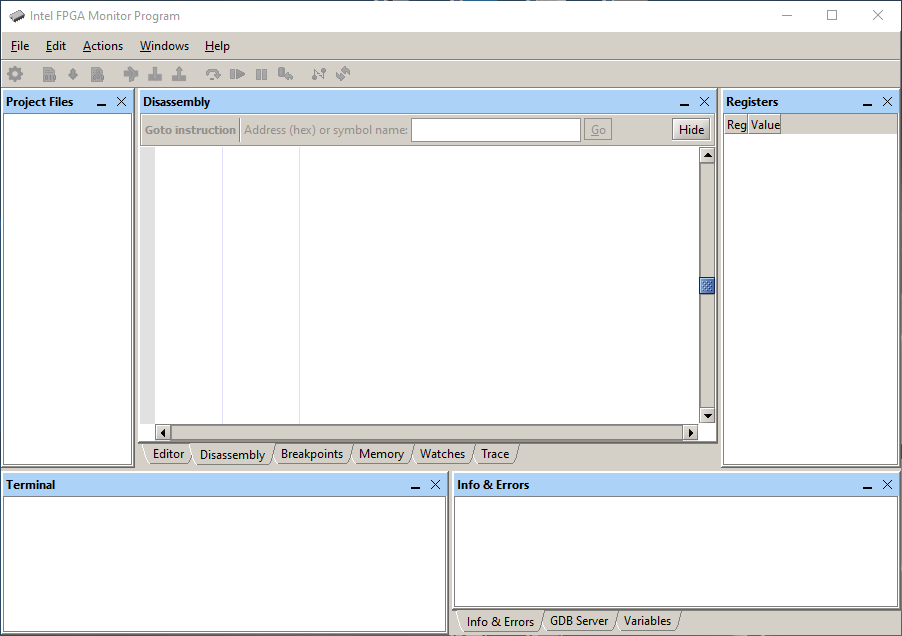
\includegraphics[scale=0.6]{screenshots/figure3.png}
   \end{center}
   \caption{The main Monitor Program display.} 
   \label{fig:AMP_maindisplay}
\end{figure}

This display consists of several windows that provide access to all of the features of the Monitor Program, which the user
selects with the computer mouse. Most of the commands 
provided by the Monitor Program can be accessed by using a set of
menus that are located below the title bar. For example, in
Figure \ref{fig:AMP_maindisplay} clicking the left mouse button on the {\sf File} command
opens the menu shown in Figure \ref{fig:AMP_filemenu}. Now, clicking the left mouse 
button on the entry {\sf New Project} begins the process of
defining a new project. Clicking on the entry {\sf Open Project}
opens an existing project. In most cases, whenever the mouse is used to select something, the left button is used. 
Hence we will not normally specify which button to press. 

\begin{figure}[H]
   \begin{center}
      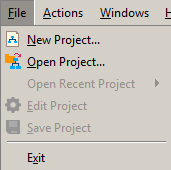
\includegraphics[scale=1]{screenshots/figure4.png}
   \end{center}
   \caption{An example of the {\sf File} menu.} 
   \label{fig:AMP_filemenu}
\end{figure}

For some commands it is necessary to access two or more menus in
sequence. In this document we use the convention 
{\sf Menu1 > Menu2 > Item} to
indicate that to select the desired command 
the user should first click the mouse button on {\sf Menu1}, 
then within this menu click on {\sf Menu2}, and then 
within {\sf Menu2} click on {\sf Item}. For example, 
{\sf File > Exit} uses the mouse to exit from the Monitor
Program. Many commands can alternatively be invoked 
by clicking on an icon displayed in the Monitor Program window. To see the command associated with an icon, position the mouse
over the icon and a tooltip will appear that displays 
the command name.

\subsection{New Project Wizard}

To start working on a new software application we have
to create a new project. Select {\sf File > New Project} to open the {\it New Project Wizard}, which leads to the screen 
in Figure \ref{fig:NPW_directoryselect}. 

\begin{figure}[H]
   \begin{center}
      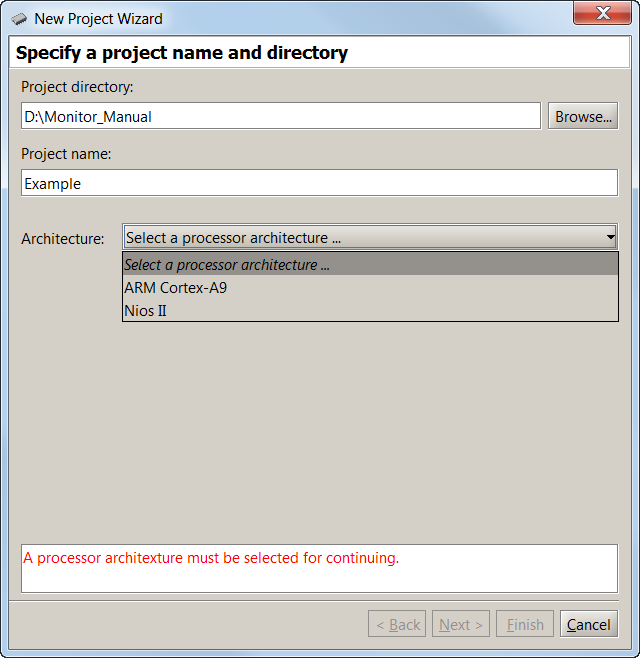
\includegraphics[scale=1]{screenshots/figure5.png}
   \end{center}
   \caption{Specifying the project directory and name.} 
   \label{fig:NPW_directoryselect}
\end{figure}


The Wizard presents a sequence of screens for
defining a new project. Each screen includes a number of dialogs, as well as a message area at the bottom of the window.  
The message area is used to display error and information messages associated with the dialogs in the window. 
Double-clicking the mouse on an error message moves the cursor
into the dialog box that contains the source of the error.


In Figure \ref{fig:NPW_directoryselect} we have specified the file system directory
{\it D:$\backslash$Monitor\_Manual} and the project 
name {\it Example}. 
If the directory specified for the project does not
already exist, a message will be displayed indicating that this
new directory will be created. To select an existing directory
by browsing through the file system, click on the {\sf Browse} button. 

{\bf Starting multiple projects in the same directory may result in unexpected behavior.}

The Monitor Program can be used with either a Nios II-based
system or an ARM-based system. The choice of a processor is made
in the window in Figure \ref{fig:NPW_directoryselect} in the box labeled Architecture.
Select the processor of your choice. 
In the discussion below we will show examples of both choices. 

\subsubsection{Specifying the Desired Hardware System}

Click {\sf Next} to advance to the window shown in Figure \ref{fig:NPW_systemselect},
which is used to specify a particular system.

\begin{figure}[H]
   \begin{center}
      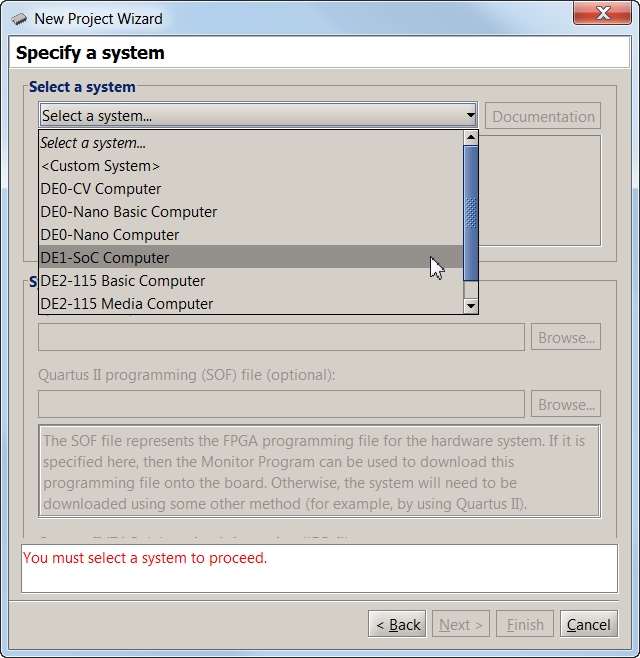
\includegraphics[scale=1]{screenshots/figure6.png}
   \end{center}
   \caption{Specifying the hardware system.} 
   \label{fig:NPW_systemselect}
\end{figure}

The drop-down list on the {\sf Select a system} pane can be used
to choose the system to be used in the project. 
The Monitor Program includes a number of prebuilt computer
systems for Intel's Development and Education boards.
Since in this document we assume that the user has access to a
DE1-SoC board, we will use a system called the 
{\it DE1-SoC Computer}. 
This computer includes a number of interfaces to 
input/output devices implemented in the FPGA fabric of the chip.
Upon selecting the DE1-SoC Computer, the screen in Figure \ref{fig:NPW_systemselect_done}
appears.

\begin{figure}[H]
   \begin{center}
      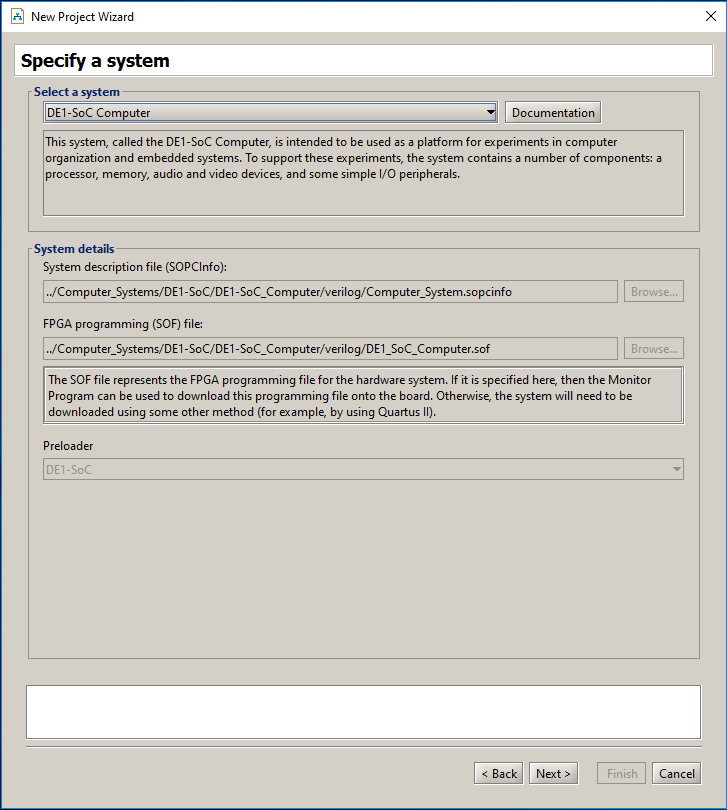
\includegraphics[scale=0.5]{screenshots/figure7.png}
   \end{center}
   \caption{The selected hardware system.} 
   \label{fig:NPW_systemselect_done}
\end{figure}

A hardware system to be implemented on the FPGA board is usually
generated by using Intel's Platform Designer tool.
Information about creating systems using Platform Designer can be found in the \emph{Introduction to the Intel Platform Designer System Integration Tool} tutorial, which is available in the University Program section of
Intel's website.

A system designed and generated by using Quartus Prime and its Platform Designer
tool is described in \emph{SOPCInfo} and \emph{SOF} files. The
former gives a high-level description of the system. 
The latter represents the FPGA
circuit that implements the designed system; this file can be downloaded into the FPGA chip on the board that is being used. 

Any system which contains a {\it Hard Processor System} (HPS) component must also specify the preloader to be run immediately following the circuit being downloaded. This preloader is used to configure the components within the HPS with the setting required for the specific board. 

The DE1-SoC Computer was created using Quartus Prime and its Platform Designer
tool. It is represented by \emph{.sopcinfo} and \emph{.sof} files
which are automaticaly included when this computer is selected.
The DE1-SoC preloader is automatically loaded.

The user may also design and implement a custom system.
If the custom system is selected, then the user must manually 
specify the \emph{.sopcinfo} and \emph{.sof} files that define
the required system in the {\sf System details} pane. If the custom system contains an HPS, the user must select their board from the preloader dropdown menu.

In the top right corner of Figure \ref{fig:NPW_systemselect_done} there is a 
{\sf Documentation} button. 
Clicking on this button opens a user guide that provides all
information needed for developing the application programs for
the DE1-SoC Computer, such as the memory map for addressing all
of the I/O devices in the system. This file can also be accessed
at a later time by using the command 
{\sf Settings > System Settings} and then
clicking on the {\sf Documentation} button.

\subsubsection{Specifying the Application Software}

In the screen of Figure \ref{fig:NPW_systemselect_done} click {\sf Next} to advance to the
screen in Figure \ref{fig:NPW_programtype}, which is used to specify the type of program
source files that are associated with the project.

\begin{figure}[H]
   \begin{center}
      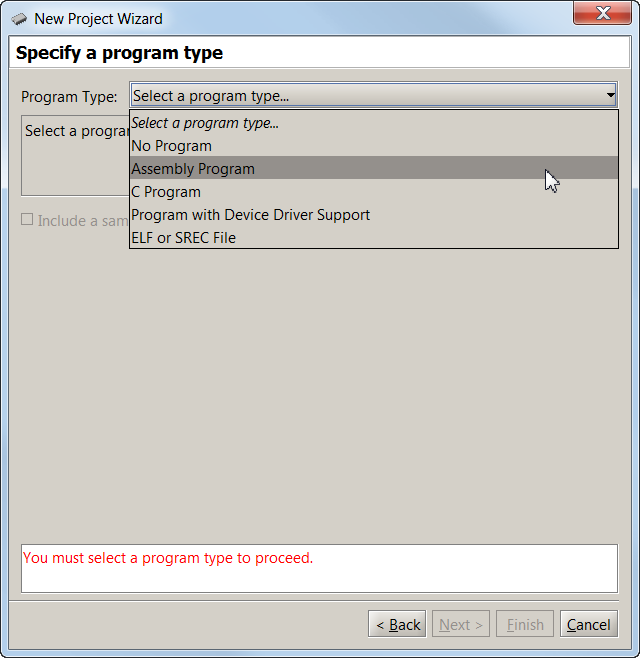
\includegraphics[scale=1]{screenshots/figure8.png}
   \end{center}
   \caption{Selecting a program type.} 
   \label{fig:NPW_programtype}
\end{figure}

The {\sf Program Type} drop-down list can be used to select one of the following program types:

\begin{itemize}
\item {\sf Assembly Program}: allows the Monitor Program to be
used with the assembly-language code
\item {\sf C Program}: allows the Monitor Program to be used with
C code
\item {\sf Program with Device Driver Support}: this is an
advanced option, which can be used to develop programs that make
use of device driver software for the I/O devices in a Nios~II
hardware system.  Programs that use this option can be written in
either assembly, C, or C++ language (or any combination). 
More information about writing programs that use device drivers
can be found in Section 18.
\item {\sf ELF or SREC File}: allows the Monitor Program to be
used with a precompiled program, in ELF, SREC or AXF format
\item {\sf No Program}: allows the Monitor Program to connect to
the hardware system on the FPGA device without first loading a
program; this can be useful if one wants to examine the current
state of some I/O devices without running an actual program.
\end{itemize}

For our example, set the program type to {\sf Assembly Program}.
When the DE1-SoC computer has been selected for the project, 
it is possible to click on the
selection {\sf Include a sample program with the project}.  
As illustrated in Figure \ref{fig:NPW_sampleprograms}, several sample 
assembly-language programs are available for this prebuilt
computer.  For our discussion select the program named 
{\it Simple Program}. This is a very simple program which
continuously reads the state of the slider switches on the
DE1-Soc board and displays their state on the red LEDs.
Click {\sf Next} to advance to the screen in Figure \ref{fig:NPW_sourcefiles}.

\begin{figure}[H]
   \begin{center}
      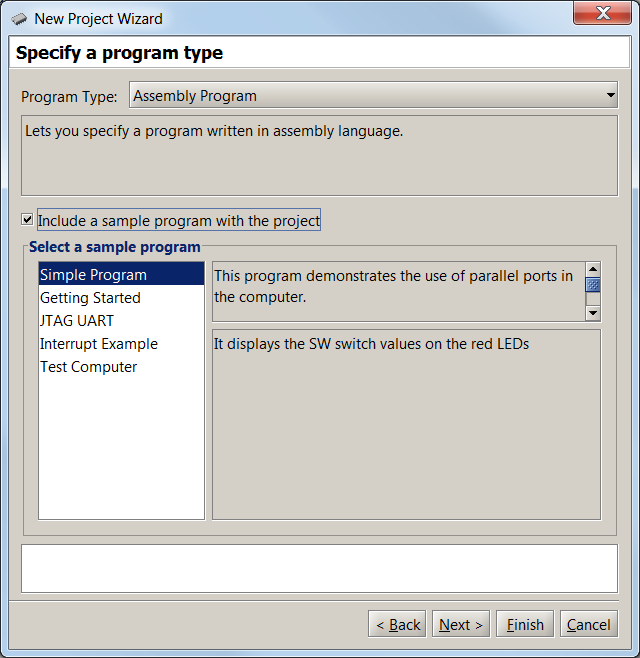
\includegraphics[scale=1]{screenshots/figure9.png}
   \end{center}
   \caption{Selecting a sample program.} 
   \label{fig:NPW_sampleprograms}
\end{figure}

\begin{figure}[H]
   \begin{center} 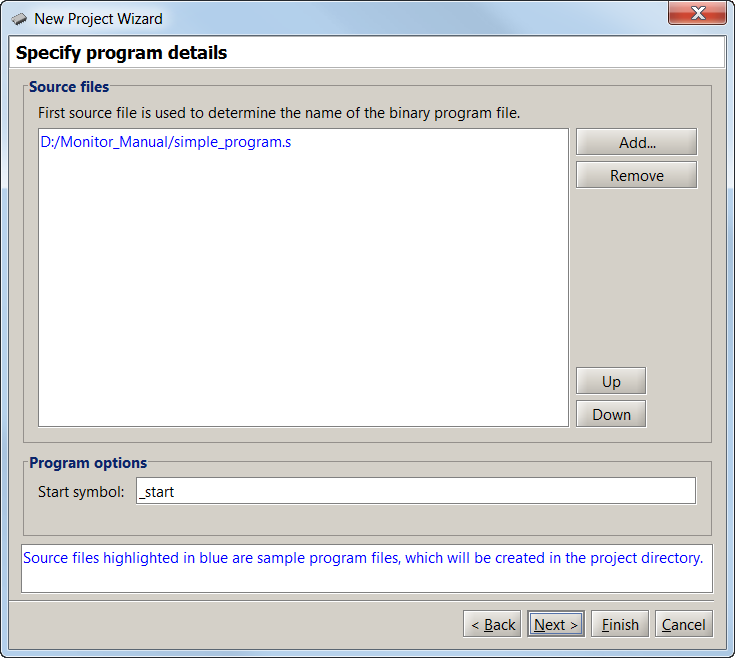
\includegraphics[scale=1]{screenshots/figure10.png}
   \end{center}
   \caption{Specifying source code files.} 
   \label{fig:NPW_sourcefiles}
\end{figure}
 
When a sample program has been
selected, the source code file(s) associated with this program
is listed in the {\sf Source files} box.  In this case, the source file is named {\it simple\_program.s}; this
file will be copied into the directory used for the project by
the Monitor Program. 
If a sample program is not used, then it is necessary to click
the {\sf Add} button and browse to select the desired source 
file(s).

Figure \ref{fig:NPW_sourcefiles} shows how it is possible to specify a label
that identifies the first instruction to be executed. 
In the {\it simple\_program.s} file, this label is called 
{\it \_start}, as indicated in the figure.

\subsubsection{System Settings}

Now, it is necessary to specify the system settings.
In the screen of Figure \ref{fig:NPW_sourcefiles}, click {\sf Next} to advance to the
window in Figure \ref{fig:NPW_systemparameters}.
This window is used to specify the connection to the FPGA board, the processor that should be used (some hardware systems may
contain multiple processors), and the terminal device.
The {\sf Host connection} drop-down list contains the physical
connection links (such as cables) that exist between the host computer and any FPGA boards connected to it. 
The processors available in the system are found in the 
{\sf Processor} drop-down list, and all 
terminal devices connected to the selected processor are displayed in the {\sf Terminal device} drop-down list. 
Terminal devices are discussed in Section 12.

Use the choices that are displayed in Figure \ref{fig:NPW_systemparameters}. If the Host Connection box is blank, make sure that 
the DE1-SoC board is connected to the host by a USB cable and
that its power is turned on. Then, press the {\sf Refresh} button and select DE-SoC [USB-1] as the desired choice.

\begin{figure}[H]
   \begin{center}
      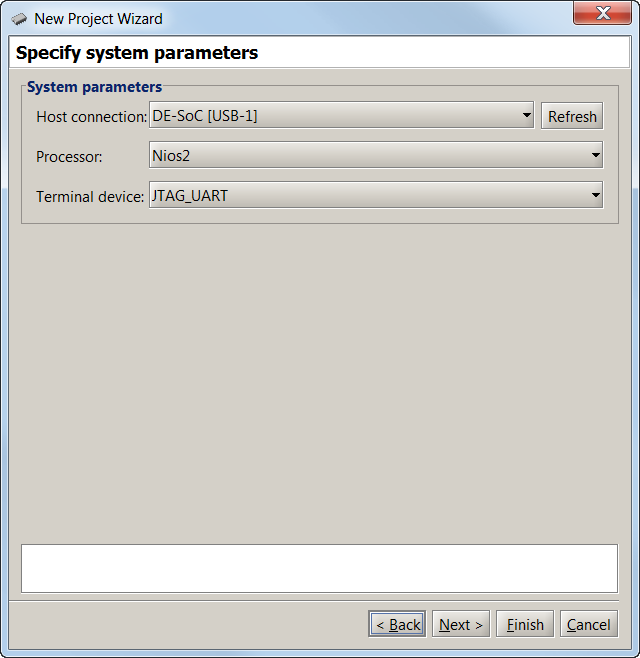
\includegraphics[scale=1]{screenshots/figure11.png}
   \end{center}
   \caption{Specifying system settings.} 
   \label{fig:NPW_systemparameters}
\end{figure}


\subsubsection{Memory Settings}

It is necessary to specify memory settings that are needed for
compiling and linking the selected application program.
Click {\sf Next} to reach the final screen for creating the new
project, shown in Figure \ref{fig:NPW_memoryoptions}. This screen is used to specify memory settings that are needed for compiling and linking the
program.

\begin{figure}[H]
   \begin{center}
      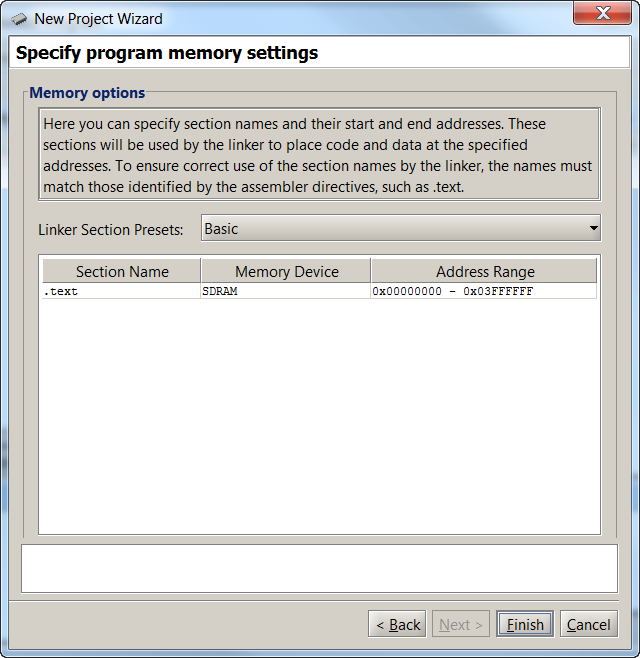
\includegraphics[scale=1]{screenshots/figure12.png}
   \end{center}
   \caption{Specifying memory settings.} 
   \label{fig:NPW_memoryoptions}
\end{figure}

There are two modes that can be selected. In the {\sf Basic}
mode, which does not provide explicitly for the use of
interrupts, the application program starts at memory address
0x00000000 as shown in the figure. A more general alternative
is to use the {\sf Interrupts} mode, which is discussed in
Section 14.  
The program in the {\it .text} section can start 
at some other address, as may be specified by the user.
To change the address, double-click on the {\it .text} entry
and change the address in the pop-up box that appears.

Clicking {\sf Save} causes the New Project Wizard to complete
the creation of the project.

{\it If you would like to continue on with the ARM version of the tutorial, click \hyperref[tut:arm_0]{here}.}

{\it If you would like to continue on with the Nios II version of the tutorial, click \hyperref[tut:nios_1]{here}.}

\clearpage
\newpage
\section{Downloading a Hardware System}
\label{tut:arm_0}

The specified hardware system must be downloaded onto the FPGA
board. In response to clicking {\sf Save} in the screen of 
Figure \ref{fig:NPW_memoryoptions}, the Monitor Program displays the prompt shown in
Figure \ref{fig:NPW_downloadprompt}. Clicking {\sf Yes} instructs the Monitor Program to
download the hardware system. It is also possible to download the
system at a later time by using the Monitor Program command
{\sf Actions > Download System}.
If the downloaded system contains more than one processor,
the Monitor Program will prompt you to halt the processors other
than the one being used for the current project. It is generally
recommended to halt the other processors because they can execute
without you knowing, resulting in unexpected behavior.

{\it To continue to the next section of the ARM tutorial, click \hyperref[tut:arm_1]{here}.}

\begin{figure}[H]
   \begin{center}
      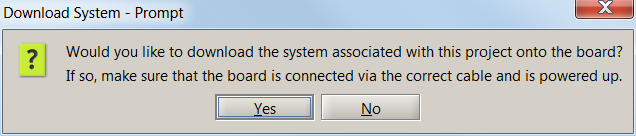
\includegraphics[scale=1]{screenshots/figure13.png}
   \end{center}
   \caption{Download the hardware system.} 
   \label{fig:NPW_downloadprompt}
\end{figure}

\subsection{Downloading a Nios~II Hardware System}
\label{tut:nios_1}

When downloading a Nios~II hardware system onto an FPGA board, 
it is important to consider the type of license that is included
in the hardware system for the processor.
The Nios~II processor uses a licensing scheme that provides two
modes of operation: 1. an evaluation mode that allows the
processor to be used with some restrictions when no
license is present, and 2. a normal mode that allows unrestricted
use when a license is present. Nios~II licenses can be purchased
from Intel, and are also available on a donated basis through
the University Program.  The prebuilt computer systems provided
with the Monitor Program, such as the DE1-SoC Computer, include a
Nios~II processor that has a license. However, if other systems
are being used with the Monitor Program, then it is
possible that a license is not present, and the Nios~II processor
may be used in the evaluation mode. In this case it is necessary
to use a different scheme, which is described in Section 21,
to download the Nios~II hardware system onto the FPGA board and activate the evaluation mode.

{\it To continue to the next section of the Nios II tutorial, click \hyperref[tut:nios_2]{here}.}


\section{Compiling and Loading the Program}

After successfully creating a project and downloading the
hardware system, the software files specified in the project can
be compiled/assembled and downloaded onto the FPGA board using
the following commands:

\begin{itemize}
\item \textsf{Actions > Compile} menu item or 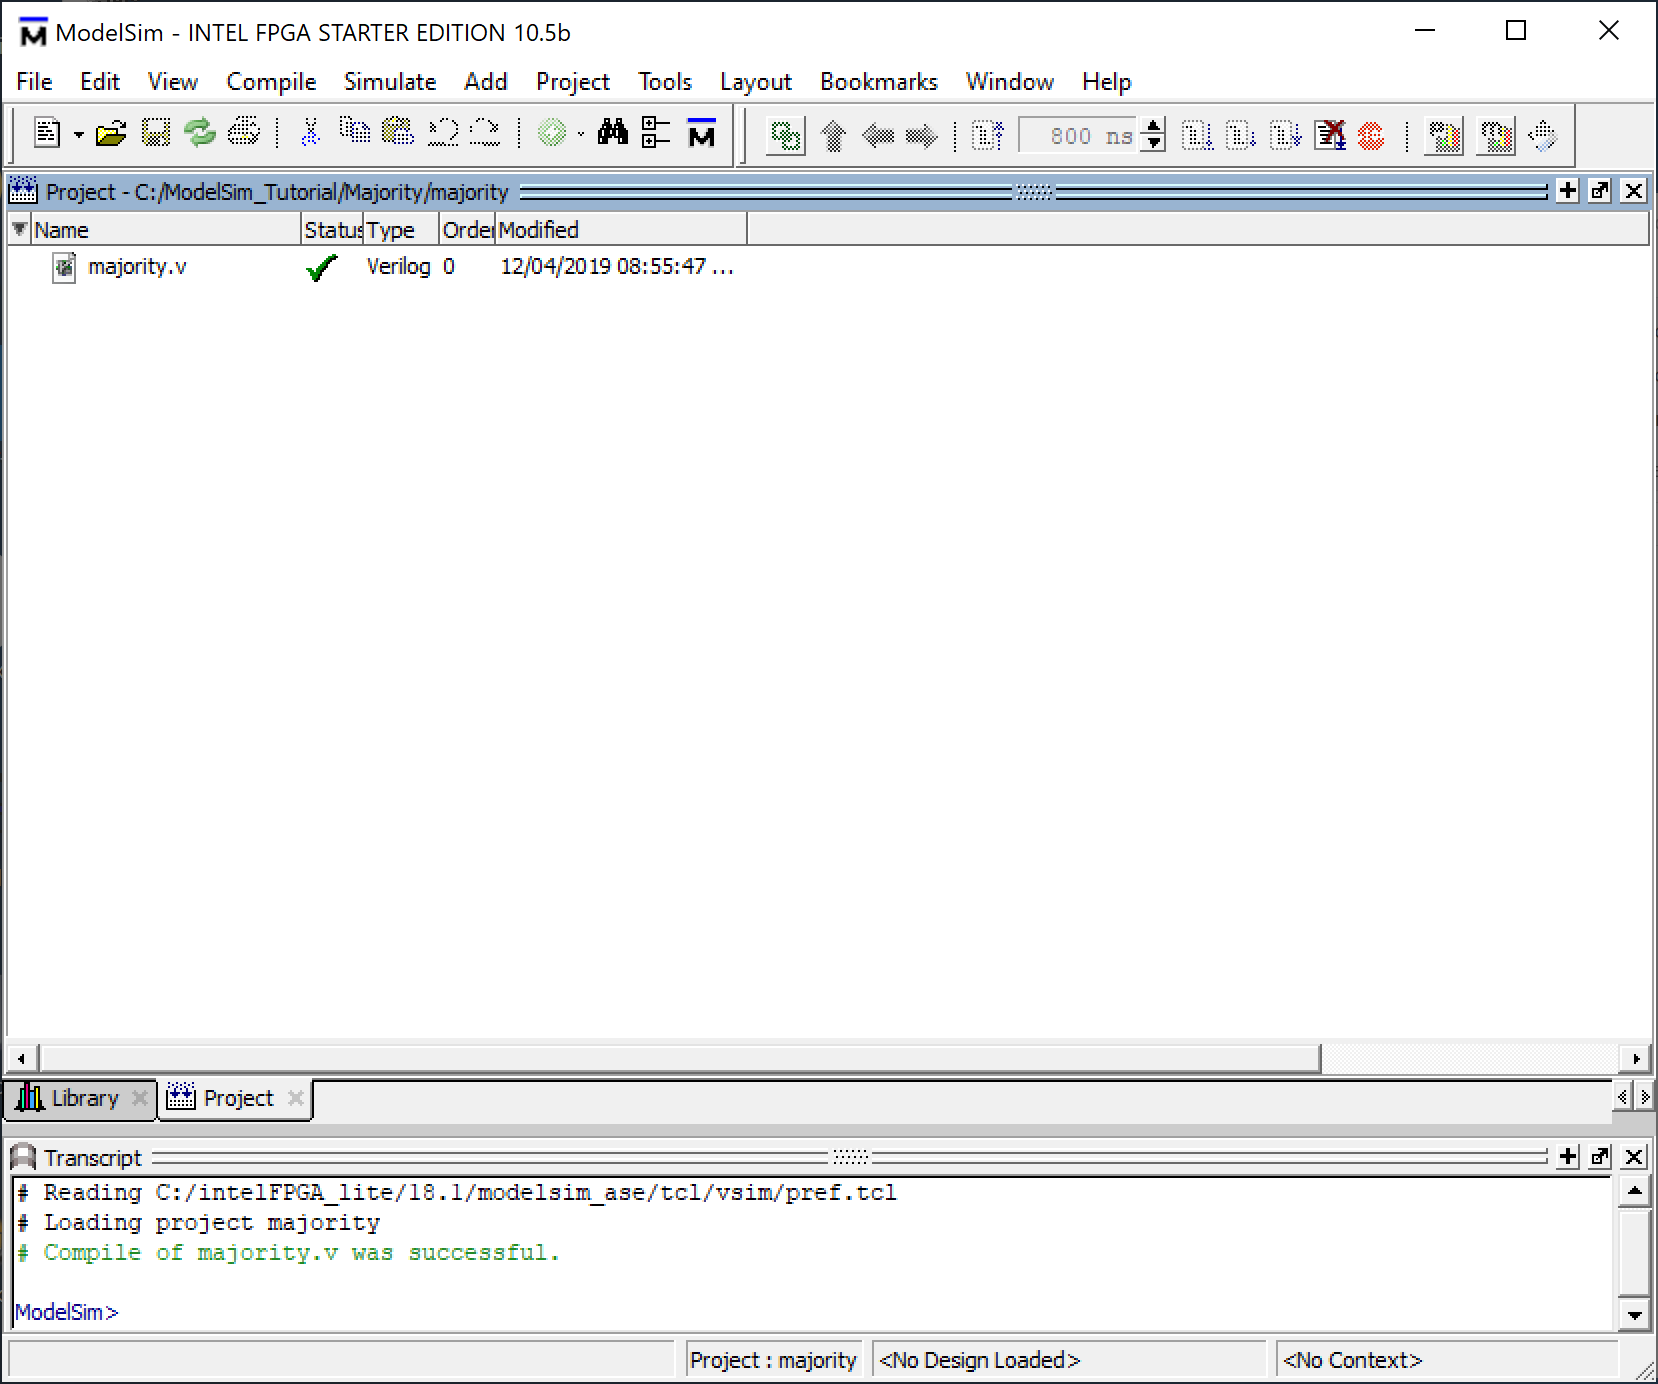
\includegraphics{toolbar/compile.png} 
icon: compiles the source files into ELF and SREC files if
Nios II is the specified processor, or into AXF and SREC files if 
ARM Cortex-A9 is the specified processor. 
Build warnings and errors will show up in the 
\textsf{Info \& Errors} window.
The generated SREC and ELF or AXF files are placed in the project's directory.

\item \textsf{Actions > Load} menu item or 
\includegraphics{toolbar/load.png} icon:
loads the compiled SREC file onto the board and begins a
debugging session in the Monitor Program. Loading progress
messages are displayed in the \textsf{Info \& Errors} window.

\item \textsf{Actions > Compile~\&~Load} menu item or 
\includegraphics{toolbar/compile_load.png}
icon: performs the operations of both compilation and loading.
\end{itemize}

As a running example, in Figure \ref{fig:NPW_sampleprograms} we selected the 
{\it Simple Program}, which is an assembly-language program
that continuously reads the state of slider switches on the 
DE1-SoC board and displays their state on the red LEDs. 
Since there is a Nios II version and an ARM version of the
program, we will discuss separately the implications of using
each version.

\subsection{The Nios II {\it Simple Program} Example}
\label{tut:nios_2}

The source code for the program is:
\begin{lstlisting}[style=defaultNiosStyle, xleftmargin=3cm]
.text
.equ     LEDs, 0xFF200000
.equ     SWITCHES, 0xFF200040
.global  _start
_start:
         movia  r2, LEDs     /* Address of red LEDs. */
         movia  r3, SWITCHES /* Address of switches. */
LOOP:    ldwio  r4, (r3)     /* Read the state of switches. */
         stwio  r4, (r2)     /* Display the state on LEDs. */
         br     LOOP
.end
\end{lstlisting}
Select the \textsf{Actions > Compile~\&~Load} menu item
or click the 
\includegraphics{toolbar/compile_load.png} icon to
begin the compilation and loading process.  
Throughout the process, messages are displayed in 
the \textsf{Info \& Errors} window. The messages should resemble
those shown in Figure \ref{fig:AMP_compilationmessages_nios}.

\begin{figure}[H]
   \begin{center}
      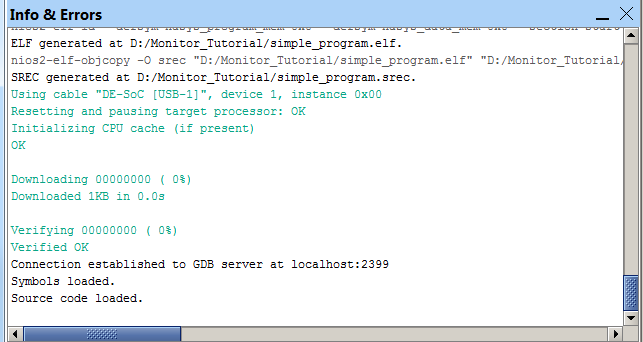
\includegraphics[scale=1]{screenshots/figure14.png}
   \end{center}
   \caption{Compilation and loading messages.} 
   \label{fig:AMP_compilationmessages_nios}
\end{figure}

After successfully completing this step, the Monitor Program display should look similar to Figure \ref{fig:AMP_afterprogramload_nios}. At this point the
processor is halted at the first instruction of the program that
has to be executed, which is highlighted in yellow shading.
The main part of the display in Figure \ref{fig:AMP_afterprogramload_nios} is called the
{\it Disassembly} window. 
It shows the machine code for the assembled program,
as well as the addresses of memory locations in which the
instructions are loaded. It also shows the assembly-language
version of the assembled instructions.

\begin{figure}[H]
   \begin{center}
      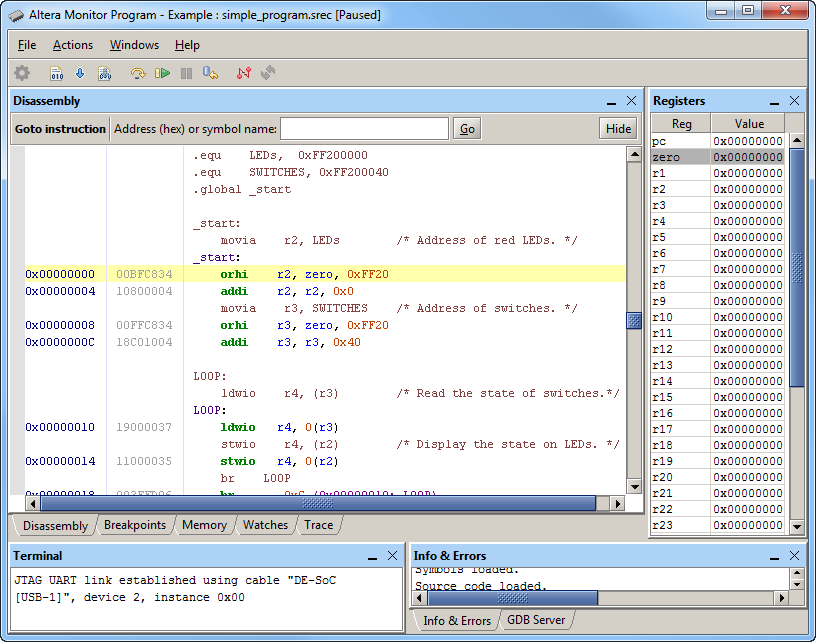
\includegraphics[scale=0.6]{screenshots/figure15.png}
   \end{center}
   \caption{The Monitor Program window after loading the program.} 
   \label{fig:AMP_afterprogramload_nios}
\end{figure}

Most instructions in a Nios II assembly-language source program
are assembled into directly-corresponding machine instructions in
the object code that is loaded into the memory for execution.
But, this is not the case with all instructions. The Nios II
assembly language provides numerous {\it pseudo-instructions},
which are often replaced by actual instructions that look
quite different but have the same effect when executed.
For instance, the pseudo-instruction
\begin{center}
movia~~~r3, SWITCHES
\end{center}
\noindent
loads into processor register r3 the memory address of the I/O
data register that is connected to the slider switches on the
board. The required address is 32 bits long. However, immediate
operands in Nios II Load instructions can be at most 16 bits
long. Therefore, as seen in Figure \ref{fig:AMP_afterprogramload_nios}, 
the second \texttt {movia} instruction is replaced with two
instructions. The instruction 
\begin{center}
orhi~~~r3, zero, 0xFF20
\end{center}
\noindent
places the immediate operand 0xFF20 into the high-order 16 bits
of register r3 and leaves the low-order 16 bits equal to zero.
The instruction
\begin{center}
addi~~~r3, r3, 0x40
\end{center}
\noindent
changes the low-order 16 bits into 0x40, thus completing in
register r3 the required address 0xFF200040.
Information about Nios~II instructions and
pseudo-instructions can be found in the tutorial
\emph{Introduction to the Intel Nios~II Soft Processor}, available in the University Program section of Intel's website.


\subsubsection{Compilation Errors}

During the process of developing software, it is likely that compilation errors will be 
encountered. Error messages from the Nios II assembler or from
the C compiler are displayed in the \textsf{Info \& Errors}
window. To see an example of a compiler error message, edit
the file {\it simple\_program.s}, which is in the project's directory, and replace the Branch instruction mnemonic 
\texttt {br} with \texttt {b}.
Recompile the project to see the error shown in Figure \ref{fig:AMP_compilererror_nios}. 
The error message indicates the type of error and it gives the
line number in the file where the error was detected. Fix the
error, and then compile and load the program again.

{\it To continue to the next section of the Nios II tutorial, click \hyperref[tut:nios_3]{here}.}

\begin{figure}[H]
   \begin{center}
      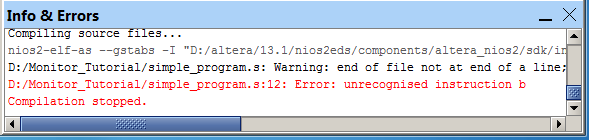
\includegraphics[scale=1]{screenshots/figure16.png}
   \end{center}
   \caption{An example of a compiler error message.} 
   \label{fig:AMP_compilererror_nios}
\end{figure}

\subsection{The ARM {\it Simple Program} Example}
\label{tut:arm_1}

The source code for the program is:

\begin{lstlisting}[style=defaultArmStyle, xleftmargin=3cm]
.text
.equ     LEDs, 0xFF200000
.equ     SWITCHES, 0xFF200040
.global  _start
_start:
         LDR   R1, =LEDs     /* Address of red LEDs. */
         LDR   R2, =SWITCHES /* Address of switches. */
LOOP:    LDR   R3, [R2]      /* Read the state of switches. */
         STR   R3, [R1]      /* Display the state on LEDs. */
         B     LOOP
.end
\end{lstlisting}

Select the \textsf{Actions > Compile~\&~Load} menu item
or click the 
\includegraphics{toolbar/compile_load.png} icon to
begin the compilation and loading process.  
Throughout the process, messages are displayed in 
the \textsf{Info \& Errors} window. The messages should resemble
those shown in Figure \ref{fig:AMP_compilationmessages_arm}.

\begin{figure}[H]
   \begin{center}
      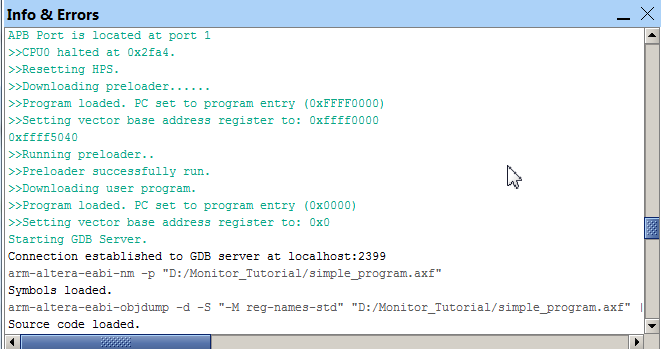
\includegraphics[scale=1]{screenshots/figure17.png}
   \end{center}
   \caption{Compilation and loading messages.} 
   \label{fig:AMP_compilationmessages_arm}
\end{figure}

After successfully completing this step, the Monitor Program display should look similar to Figure \ref{fig: AMP_afterprogramload_arm}. At this point the
processor is halted at the first instruction of the program that
has to be executed, which is highlighted in yellow shading.
The main part of the display in Figure \ref{fig: AMP_afterprogramload_arm} is called the
{\it Disassembly} window. 
It shows the machine code for the assembled program,
as well as the addresses of memory locations in which the
instructions are loaded. It also shows the assembly-language
version of the assembled instructions.


\begin{figure}[H]
   \begin{center}
      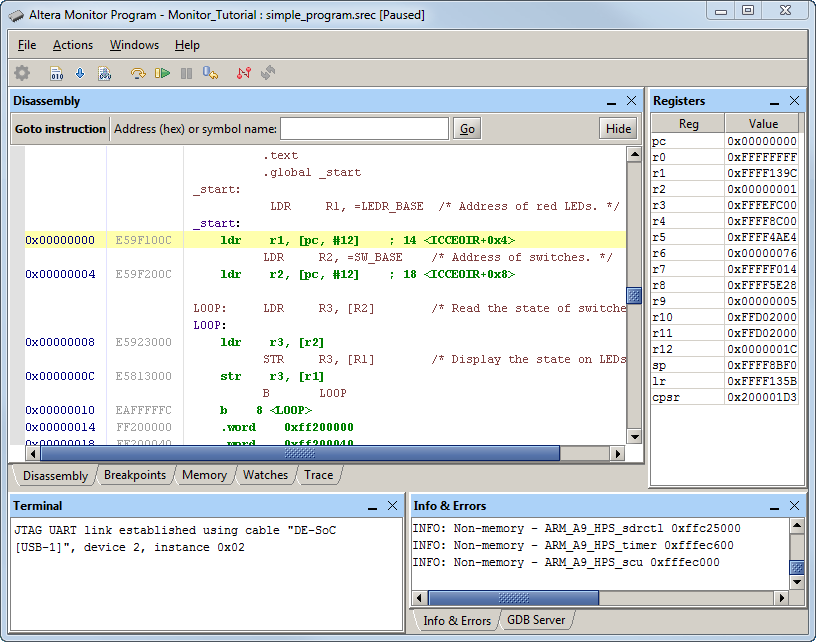
\includegraphics[scale=0.6]{screenshots/figure18.png}
   \end{center}
   \caption{The Monitor Program window after loading the program.} 
   \label{fig: AMP_afterprogramload_arm}
\end{figure}


Most instructions in an ARM assembly-language source program are
assembled into directly-corresponding machine instructions in
the object code that is loaded into the memory for execution.
However, this is not the case with all instructions. The ARM
assembly language provides numerous {\it pseudo-instructions},
which are often replaced by actual instructions that look
quite different but have the same effect when executed.
For instance, the instruction 
\begin{center}
LDR~~~R1, =LEDs
\end{center}
\noindent
loads into processor register R1 the memory address of the I/O
data register that is connected to the LEDs on the board.
As seen in Figure \ref{fig: AMP_afterprogramload_arm}, this instruction is replaced with the 
instruction 
\begin{center}
LDR~~~R1, [PC, \#12]
\end{center}
\noindent
in the assembled code. Since Load instructions in the ARM
processor cannot specify an immediate operand that is 32 bits 
long, the address 0xFF200000 is placed in the {\it literal pool}
after the last instruction in the program. Then, the implemented
LDR instruction uses the {\it Relative} addressing mode (which
is the {\it Offset} addressing mode that uses the Program Counter
as the base register) to access the desired address value. Observe that the offset used in this case is 12 bytes.
The reason is that the ARM processor prefetches two instructions
to facilitate pipelined execution of the program. 
When an instruction is prefetched, the Program Counter is
incremented by four. Thus, in our example, the updated
PC contents will be 0x08 when the first LDR instruction is
being executed. Then, the offset of 12 bytes leads to the memory
location 0x14.
 
Note that in an ARM assembly-language program it is possible to
use both upper- and lower-case letters to denote register names
and instruction mnemonics.

Information about the ARM instructions, addressing modes and
literal pools can be found in the tutorial
{\it Introduction to the ARM Processor Using Intel Toolchain},
which is available in the University Program section of Intel's
website. 

\subsubsection{Compilation Errors}

During the process of developing software, it is likely that compilation errors will be 
encountered. Error messages from the ARM assembler or from the C compiler are displayed in the \textsf{Info \& Errors} window. 
To see an example of a compiler error message, edit
the file {\it simple\_program.s}, which is in the project's directory, and replace the mnemonic STR with ST.
Recompile the project to see the error shown in Figure \ref{fig:AMP_compilererror_arm}. 
The error message indicates the type of error and it gives the
line number in the file where the error was detected. Fix the
error, and then compile and load the program again.

{\it To continue to the next section of the ARM tutorial, click \hyperref[tut:arm_2]{here}.}

\begin{figure}[H]
   \begin{center}
      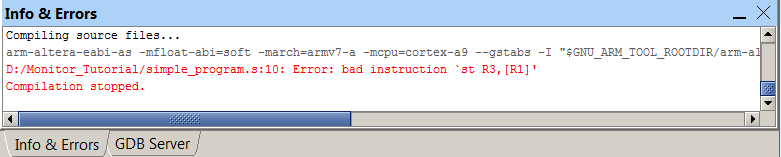
\includegraphics[scale=1]{screenshots/figure19.png}
   \end{center}
   \caption{An example of a compiler error message.} 
   \label{fig:AMP_compilererror_arm}
\end{figure}

\section{Running the Program}

As mentioned in the previous section, the processor is halted at
the first instruction after the program has been loaded. 
To run the program, select the \textsf{Actions > Continue} menu
item or click the 
\includegraphics{toolbar/continue.png} icon.  The {\it simple\_program} continuously displays the current
values of DE1-SoC board's slider switches on the red LEDs.
The \textsf{Continue} command runs the program indefinitely.
To force the program to halt,
select the \textsf{Actions > Stop} command, or click the

\includegraphics{toolbar/stop.png} icon. This command causes the
processor to halt at the instruction to be executed next, and
returns control to the Monitor Program.

\subsection{The Nios II Example - continued} 
\label{tut:nios_3}

Figure \ref{fig:AMP_stoppedprogram_nios} illustrates what the display may look like when
our {\it Simple Program} is halted by using the 
{\sf Stop} command. 
The display highlights in yellow the next program instruction to
be executed, which is at address \texttt {0x00000014},
and highlights in red the values in the processor
registers that have changed since the last program stoppage.
Other screens in the Monitor Program are also updated, which will
be described in later parts of this manual.

\begin{figure}[H]
   \begin{center}
      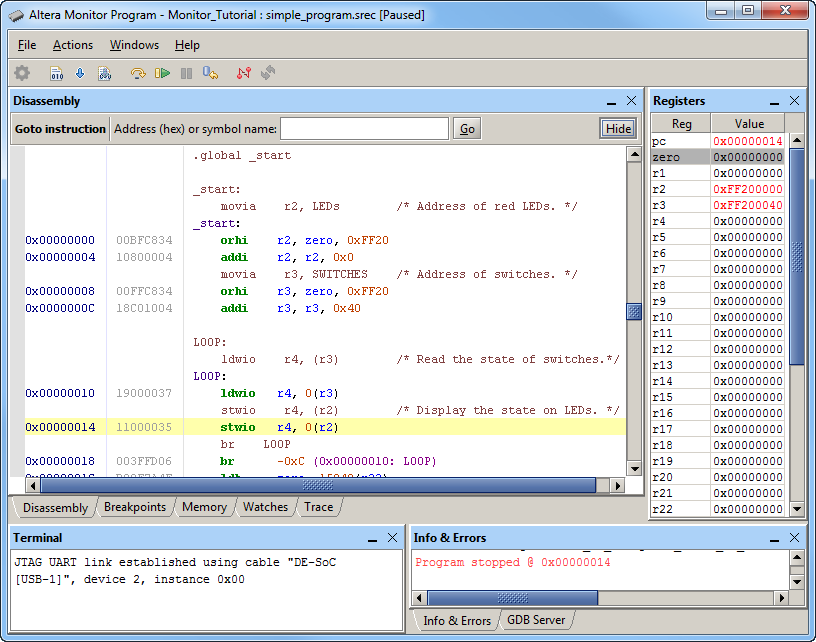
\includegraphics[scale=0.6]{screenshots/figure20.png}
   \end{center}
   \caption{The Monitor Program display after the program has been stopped.} 
   \label{fig:AMP_stoppedprogram_nios}
\end{figure}

The Disassembly window shows the machine instructions for 
our program.
The leftmost column in the window gives the memory addresses,
the middle column displays the machine code at these addresses,
and the rightmost column shows both the original source code for
the instruction, in a brown color, and the disassembled view of
the machine code that is stored in memory, in a green color.

The Disassembly window can be configured to display less information on the screen, such as 
not showing the assembly-language instructions or not showing the machine encoding of the instructions. These choices can 
be made by right-clicking on the Disassembly window and selecting
the appropriate menu item, as indicated in Figure \ref{fig:AMP_disassemblyoptions_nios}.

\begin{figure}[H]
   \begin{center}
      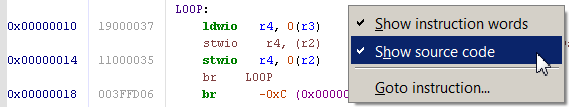
\includegraphics[scale=1]{screenshots/figure21.png}
   \end{center}
   \caption{Display options for the Disassembly window.} 
   \label{fig:AMP_disassemblyoptions_nios}
\end{figure}

Different parts of memory can be displayed by scrolling, 
using either the vertical scrollbar on the right side of the Disassembly window or a mouse scroll wheel.
It is also possible to go to a different region of memory by 
using the \textsf{Goto instruction} panel 
at the top of the Disassembly window, or by using the command \textsf{Actions > Goto instruction}.  The instruction address
provided for the {\sf Goto} command must be a multiple of four,
because Nios II instructions are word-aligned.

{\it To continue to the next section of the Nios II tutorial, click \hyperref[tut:nios_4]{here}.}

\subsection{The ARM Example - continued}
\label{tut:arm_2}

Figure \ref{fig:AMP_stoppedprogram_arm} shows an example of what the display may look like when
the program is halted by using the {\sf Stop} command. 
The display highlights in yellow the next program instruction to
be executed, which is at address \texttt {0x0000000C},
and highlights in red the values in the processor
registers that have changed since the last program stoppage.
Other screens in the Monitor Program are also updated, which will
be described in later parts of this manual.

\begin{figure}[H]
   \begin{center}
      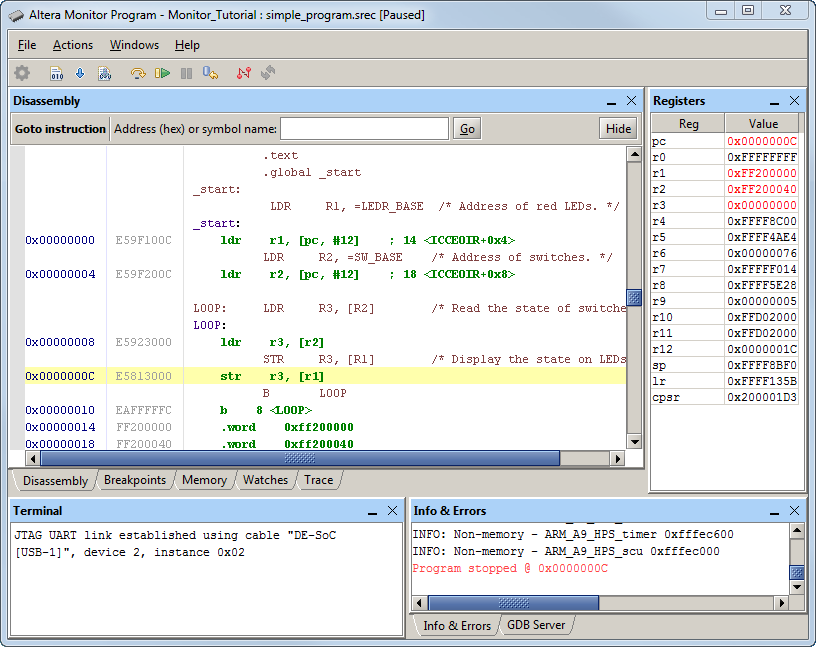
\includegraphics[scale=0.6]{screenshots/figure22.png}
   \end{center}
   \caption{The Monitor Program display after the program has been stopped.} 
   \label{fig:AMP_stoppedprogram_arm}
\end{figure}

The Disassembly window shows the machine
instructions for our program.
The leftmost column in the window gives the memory addresses,
the middle column displays the machine code at these addresses,
and the rightmost column shows the corresponding
assembly-language instructions.

The Disassembly window can be configured to display less information on the screen, such as 
not showing the assembly-language instructions or not showing the machine encoding of the instructions. These choices can 
be made by right-clicking on the Disassembly window and selecting
the appropriate menu item, as shown in Figure \ref{fig:AMP_disassemblyoptions_arm}.

\begin{figure}[H]
   \begin{center}
      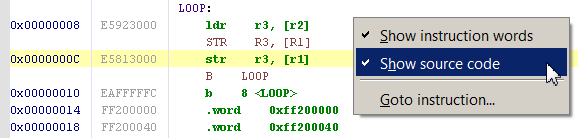
\includegraphics[scale=1]{screenshots/figure23.png}
   \end{center}
   \caption{Display options for the Disassembly window.} 
   \label{fig:AMP_disassemblyoptions_arm}
\end{figure}


Different parts of memory can be displayed by scrolling, 
using either the vertical scrollbar on the right side of the Disassembly window or a mouse scroll wheel.
It is also possible to go to a different region of memory by 
using the \textsf{Goto instruction} panel 
at the top of the Disassembly window, or by using the command \textsf{Actions > Goto instruction}.  The instruction address
provided for the {\sf Goto} command must be a multiple of four,
because ARM instructions are word-aligned. 

{\it To continue to the next section of the ARM tutorial, click \hyperref[tut:arm_3]{here}.}

\section{Single Stepping Program Instructions}

When debugging a program, it is often very useful to be able
to single step through the program and observe the effect of
executing each instruction. 
The Monitor Program has the ability to perform single-step
operations. Each single step consists of executing a single
machine instruction and then returning control to the Monitor
Program. If the source code of the program being debugged is
written in the C language, then each individual single step will
still correspond to one assembly-language (machine) instruction
generated from the C code. 

The single-step operation is invoked by selecting the
\textsf{Actions > Single step} menu item or by clicking on the 
\includegraphics{toolbar/singlestep.png} icon. The 
instruction that is executed by the processor is the
one highlighted in yellow in the \textsf{Disassembly} window.
Consider our {\it simple\_program} example. You can go to the
first instruction of the program, which has the label 
{\it \_start}, by selecting \textsf{Actions > Restart} 
menu item or by clicking  
the 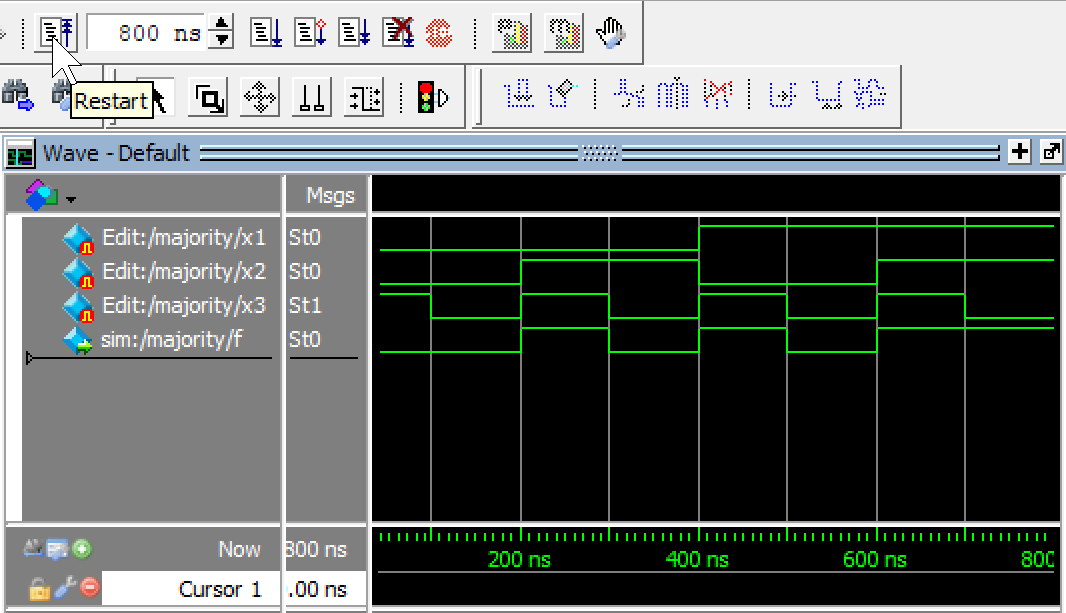
\includegraphics{toolbar/restart.png} icon. If the program is
running, it must first be halted before the restart 
command can be performed.
The restart command loads into the Program Counter the address of
the first instruction, thus causing the execution to start at
this point in the program.
Now, single step through the program and observe the displayed 
changes. Note that the register values are indicated in red when
they change as a result of executing the last instruction.

In a program that contains subroutines it is possible to step
over an entire subroutine by using the
{\sf Step Over Subroutine} command in the {\sf Actions} menu.
This command performs a normal single step, unless the current
instruction is a Call instruction, in which case the program will
run until the called subroutine is completed.


\section{Using Breakpoints}

An {\it instruction breakpoint} provides a means of stopping the
execution of a program when it reaches an instruction at a
specific address.  A breakpoint can be set as follows:

\begin{enumerate}
\item In the Disassembly window, scroll to display the instruction that will have the breakpoint. 

\item Click on the gray bar to the left of the address
for this instruction. 
The Monitor Program will display a red dot next to the address
to show that a breakpoint has been set. 
Clicking the same location again removes the breakpoint.
\end{enumerate}

If source level debugging is enabled, a {\it source breakpoint} can also be set
at a line of source code through the {\sf Editor} window. This will stop
the execution of a program when it reaches an instruction that corresponds
to that line of source code. Note that each line of source code may correspond
to multiple different lines of assembly instructions that are not necessarily contiguous.
Additionally, trying to set breakpoints by clicking to the right of certain
source code lines will sometimes not produce any result. This is because there are some lines of 
source code that do not correspond to any lines of assembly code, and the {\productNameMed}
will not let you set breakpoints at these lines of source code.

Once the instruction breakpoint has been set, run the program.
The breakpoint will trigger when the Program Counter value equals
the address of the instruction for which the breakpoint is set.
Control then returns to the Monitor Program,
and the Disassembly window highlights in a yellow color the
instruction at the breakpoint. A corresponding message is shown
in the {\sf Info \& Errors} pane.


\subsection{Using the Breakpoints Window}

Above we showed how breakpoints can be set using the Disassembly
window. Another way to set breakpoints is to click on the 
{\sf Breakpoints} tab to reach the window depicted in Figure \ref{fig:AMP_breakpointswindow}.
This window supports three 
types of breakpoints in addition to the instruction breakpoint:
{\it read watchpoint}, {\it write watchpoint}, and 
{\it access watchpoint}, as follows:

\begin{itemize}
\item Read watchpoint - the processor is halted when a read
operation is performed on a specific address.
\item Write watchpoint - the processor is halted when a write
operation is performed on a specific address.
\item Access watchpoint - the processor is halted when a read or
write operation is performed on a specific address.
\end{itemize}


\begin{figure}[H]
   \begin{center}
      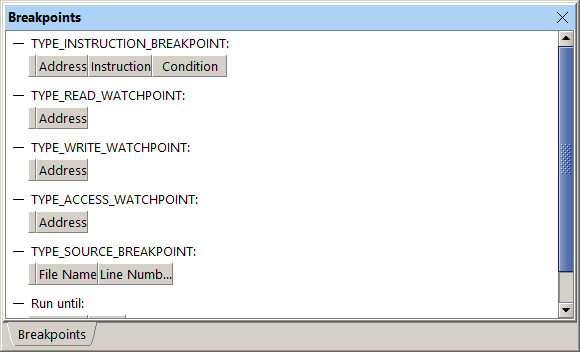
\includegraphics[scale=0.6]{screenshots/figure24.png}
   \end{center}
   \caption{The Breakpoints window.} 
   \label{fig:AMP_breakpointswindow}
\end{figure}

A breakpoint can be created by right-clicking in
a grey box under the label {\sf Instruction breakpoint},
selecting {\sf Add} in the pop-up box and then specifying the
address of an instruction. A breakpoint can be
deleted by unchecking the box beside its address.

Setting a read, write, or access watchpoint is done by
right-clicking on the appropriate box in the Breakpoints window
and specifying the desired address.

The Monitor Program also supports {\it conditional breakpoints},
which trigger only when user-specified conditions are met.
There are two possibilities:
\begin{enumerate}
\item A condition can be attached to an instruction breakpoint,
in which case the execution of the program will be halted at the
address specified in the breakpoint after the required condition
is met. Double-clicking in the {\sf Condition} box for
an instruction breakpoint leads to an
{\sf Edit breakpoint condition} dialog depicted in Figure \ref{fig:AMP_editbreakpointcondition},
in which the required condition is specified.

\begin{figure}[H]
   \begin{center}
      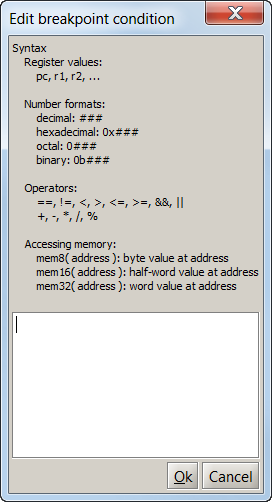
\includegraphics[scale=1]{screenshots/figure25.png}
   \end{center}
   \caption{The Edit Breakpoint Condition dialog.} 
   \label{fig:AMP_editbreakpointcondition}
\end{figure}
~\\

\begin{figure}[H]
   \begin{center}
      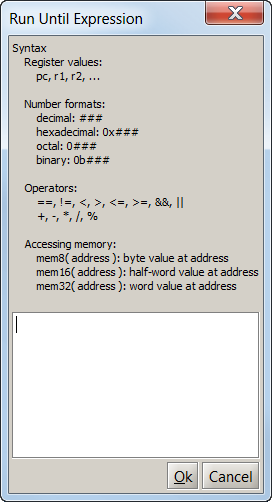
\includegraphics[scale=1]{screenshots/figure26.png}
   \end{center}
   \caption{The Run Until Expression dialog.} 
   \label{fig:AMP_rununtilexpression}
\end{figure}

\newpage 
\item A stand-alone condition can be specified in
the {\sf Run until} box, in which case the execution of the
program will be halted at the instruction that caused the
required condition to be met. 
Double-clicking in the empty box {\it under} the label 
{\sf Condition} in Figure \ref{fig:AMP_breakpointswindow} opens a 
{\sf Run Until Expression} dialog shown in Figure \ref{fig:AMP_rununtilexpression}, in which
the required condition is specified.

\end{enumerate}


\subsection{The Nios II Example - continued}
\label{tut:nios_4}

Figure \ref{fig:AMP_breakpoints_nios} shows how the Breakpoints window can be used to set
a breakpoint at the Branch instruction at address 
\texttt{0x00000018} in our {\it simple\_program}. This breakpoint can also be set in the Disassembly window by simply
clicking on the gray bar to the left of the address for this
instruction. Setting this breakpoint produces the image shown in Figure \ref{fig:AMP_breakpointexample_nios}. The breakpoint can be removed by clicking on the red
dot.
~\\

\begin{figure}[H]
   \begin{center}
      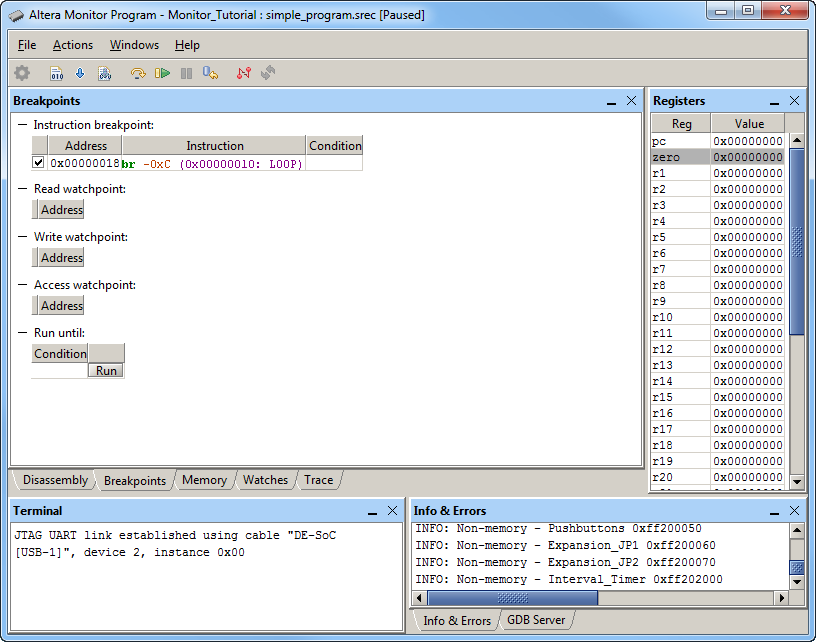
\includegraphics[scale=0.6]{screenshots/figure27.png}
   \end{center}
   \caption{The Breakpoints window for a Nios II program.} 
   \label{fig:AMP_breakpoints_nios}
\end{figure}

\begin{figure}[H]
   \begin{center}
      
\includegraphics[scale=0.6]{screenshots/figure28.png}
   \end{center}
   \caption{A breakpoint in the example Nios II program.} 
   \label{fig:AMP_breakpointexample_nios}
\end{figure}

The breakpoint can be made conditional by double-clicking in
the {\sf Condition} box in Figure \ref{fig:AMP_breakpoints_nios}, which would display the
Edit Breakpoint Condition dialog of Figure \ref{fig:AMP_editbreakpointcondition}, and entering a
desired condition. For example, suppose that we want to stop the
execution of the program when the contents of register r4
become equal to 5. Then, the required condition is
\texttt{r4 == 5}. Upon setting this condition, the breakpoint
is activated only when r4 contains the value 5.
Thus, running this program causes the 
LEDs to display the current state of the slider switches as these
switches are set to different patterns. But, when the selected
pattern is 0x005, the conditional breakpoint will stop the
execution of the program upon reaching the Branch instruction
at address \texttt{0x00000018}. 
The program can be run again by selecting the 
\textsf{Actions > Continue} menu item or by clicking the 
\includegraphics{toolbar/continue.png} icon.  
Note that the image in Figure \ref{fig:AMP_breakpointexample_nios} will remain the same whether
or not a condition has been attached to this breakpoint.

\newpage 
Next, consider the possibility of creating a breakpoint with a
stand-alone condition. This can be done by using the 
{\sf Run until} feature in the Breakpoints window, by
double-clicking in the empty box under the label {\sf Condition}
which leads to the {\sf Run Until Expression} dialog.
Entering the same condition as above, namely \texttt{r4 == 5},
produces the image in Figure \ref{fig:AMP_rununtilexpression_nios}.

\begin{figure}[H]
   \begin{center}
      
\includegraphics[scale=1]{screenshots/figure29.png}
   \end{center}
   \caption{The Run Until Expression dialog for the Nios II example.} 
   \label{fig:AMP_rununtilexpression_nios}
\end{figure}

This breakpoint is not associated with a specific instruction. It
will halt the execution of the program as soon as the contents
of r4 become equal to 5.
Since this breakpoint is not associated with a specific
instruction, there would be no red dot displayed in the
Disassembly window in Figure \ref{fig:AMP_breakpointexample_nios}. 

When a stand-alone condition is specified in the {\sf Run until}
box, then the Run button associated with this box must be used to
run the program, rather than the normal {\sf Actions > Continue} command or the 
\includegraphics{toolbar/continue.png} icon.   

{\it To continue to the next section of the Nios II tutorial, click \hyperref[tut:nios_5]{here}.}

\newpage
\subsection{The ARM Example - continued}
\label{tut:arm_3}

Figure \ref{fig:AMP_breakpoints_arm} shows how the Breakpoints window can be used to set
a breakpoint at the Branch instruction at address 
\texttt{0x00000010} in our {\it simple\_program}. This breakpoint can also be set in the Disassembly window by simply
clicking on the gray bar to the left of the address for this
instruction. Setting this breakpoint produces the image shown in Figure \ref{fig:AMP_breakpointexample_arm}. The breakpoint can be removed by clicking on the red
dot.
~\\

\begin{figure}[H]
   \begin{center}
      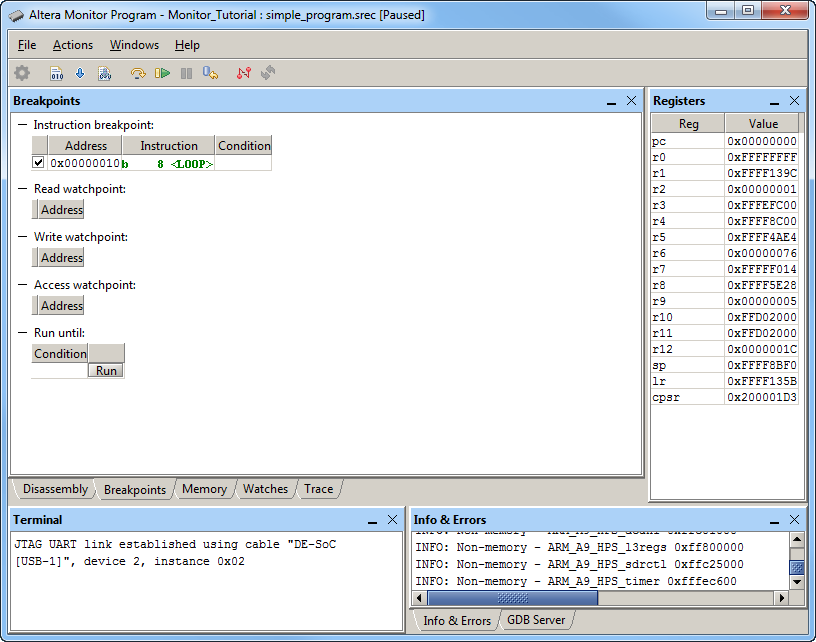
\includegraphics[scale=0.6]{screenshots/figure30.png}
   \end{center}
   \caption{The Breakpoints window for an ARM program.} 
   \label{fig:AMP_breakpoints_arm}
\end{figure}

\begin{figure}[H]
   \begin{center}
      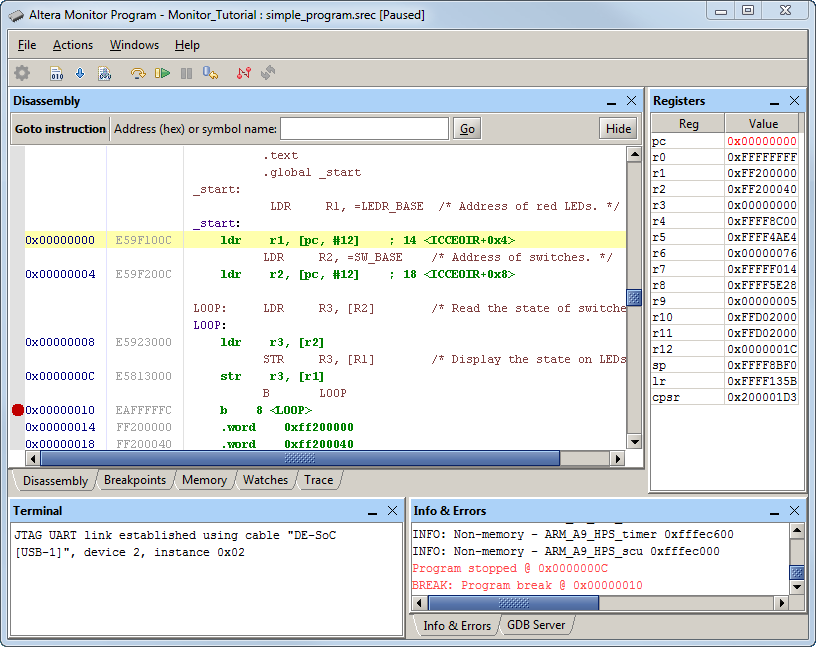
\includegraphics[scale=0.6]{screenshots/figure31.png}
   \end{center}
   \caption{A breakpoint in the example ARM program.} 
   \label{fig:AMP_breakpointexample_arm}
\end{figure}

The breakpoint can be made conditional by double-clicking in
the {\sf Condition} box in Figure \ref{fig:AMP_breakpoints_arm}, which would display the
Edit Breakpoint Condition dialog of Figure \ref{fig:AMP_editbreakpointcondition}, and entering a
desired condition. For example, suppose that we want to stop the
execution of the program when the contents of register R3
become equal to 5. Then, the required condition is
\texttt{R3 == 5}. Upon setting this condition, the breakpoint
is activated only when R3 contains the value 5.
Thus, running this program causes the 
LEDs to display the current state of the slider switches as these
switches are set to different patterns. But, when the selected
pattern is 0x005, the conditional breakpoint will stop the
execution of the program upon reaching the Branch instruction
at address \texttt{0x00000010}. 
The program can be run again by selecting the 
\textsf{Actions > Continue} menu item or by clicking the 
\includegraphics{toolbar/continue.png} icon.  
Note that the image in Figure \ref{fig:AMP_breakpointexample_arm} will remain the same whether
or not a condition has been attached to this breakpoint.

\newpage 
Next, consider the possibility of creating a breakpoint with a
stand-alone condition. This can be done by using the 
{\sf Run until} feature in the Breakpoints window, by
double-clicking in the empty box under the label {\sf Condition}
which leads to the {\sf Run Until Expression} dialog.
Entering the same condition as above, namely \texttt{R3 == 5},
produces the image in Figure \ref{fig:AMP_rununtilexpression_arm}.

\begin{figure}[H]
   \begin{center}
      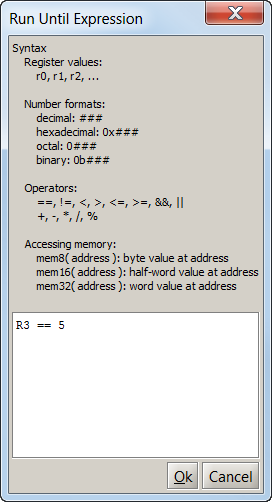
\includegraphics[scale=1]{screenshots/figure32.png}
   \end{center}
   \caption{The Run Until Expression dialog for the ARM example.} 
   \label{fig:AMP_rununtilexpression_arm}
\end{figure}

This breakpoint is not associated with a specific instruction. It
will halt the execution of the program as soon as the contents
of R3 become equal to 5.
Since this breakpoint is not associated with a specific
instruction, there would be no red dot displayed in the
Disassembly window in Figure \ref{fig:AMP_breakpointexample_arm}. 

When a stand-alone condition is specified in the {\sf Run until}
box, then the Run button associated with this box must be used to
run the program, rather than the normal {\sf Actions > Continue} command or the 
\includegraphics{toolbar/continue.png} icon.  

{\it To continue to the next section of the ARM tutorial, click \hyperref[tut:arm_4]{here}.}  

\clearpage
\newpage
\section{Using the Registers Window}

The \textsf{Registers} window on the right-hand side of the
Monitor Program display shows the values of processor registers.
It also allows the user to edit most of the register values. 
The number format in which the register values are displayed
can be changed by right-clicking in the \textsf{Registers}
window and selecting the desired format, as illustrated in 
Figure \ref{fig:AMP_registeroptions}.

\begin{figure}[H]
   \begin{center}
      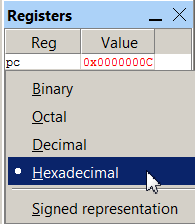
\includegraphics[scale=1]{screenshots/figure33.png}
   \end{center}
   \caption{Setting the number format for displaying register values.} 
   \label{fig:AMP_registeroptions}
\end{figure}

Each time program execution is halted, the Monitor Program
updates the register values and highlights any changes in red.
The user can edit the register values while the program is
halted. Any edits made are visible to the processor when the
program's execution is resumed.

\subsection{The Nios II Example - continued}
\label{tut:nios_5}

As an example of editing a register value, set the slider
switches on the DE1-SoC board to some pattern of 0s and 1s.
Run the {\it simple\_program} and observe that the LEDs display
the selected pattern. Next, stop the execution of the program
and set a breakpoint at the Store instruction
at address \texttt{0x00000014}. Run the program and
after the execution stops at the breakpoint, observe that the
value in register r4 corresponds to the current setting of the
slider switches. 
Now,  as indicated in Figure \ref{fig:AMP_editregister_nios}, double-click on the contents of
register r4 and change them to the value FFF.  
Press \textsf{Enter} on the computer keyboard, or click away from
the register value to apply the edit. 
Then, single-step the program to see that all LEDs will be
turned on. 

{\it To continue to the next section of the Nios II tutorial, click \hyperref[tut:nios_6]{here}.}

\begin{figure}[H]
   \begin{center}
      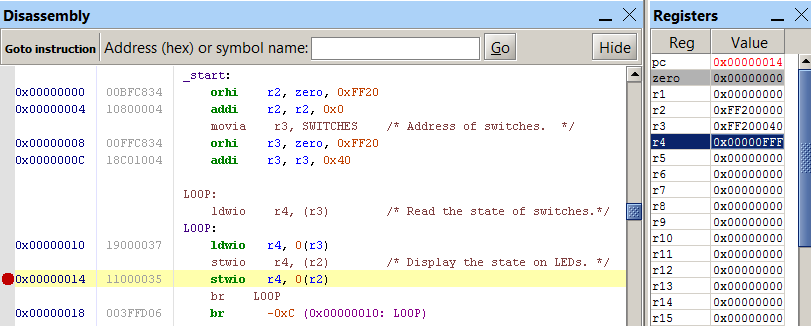
\includegraphics[scale=1]{screenshots/figure34.png}
   \end{center}
   \caption{Editing a register value.} 
   \label{fig:AMP_editregister_nios}
\end{figure}


\subsection{The ARM Example - continued}
\label{tut:arm_4}

As an example of editing a register value, set the slider
switches on the DE1-SoC board to some pattern of 0s and 1s.
Run the {\it simple\_program} and observe that the LEDs display
the selected pattern. Next, stop the execution of the program
and set a breakpoint at the Store instruction
at address \texttt{0x0000000C}. Run the program and
after the execution stops at the breakpoint, observe that the
value in register R3 corresponds to the current setting of the
slider switches. 
Now,  as indicated in Figure \ref{fig:AMP_editregister_arm}, double-click on the contents of
register R3 and change them to the value FFF.  
Press \textsf{Enter} on the computer keyboard, or click away from
the register value to apply the edit. 
Then, single-step the program to see that all LEDs will be
turned on. 

{\it To continue to the next section of the ARM tutorial, click \hyperref[tut:arm_5]{here}.}

\begin{figure}[H]
   \begin{center}
      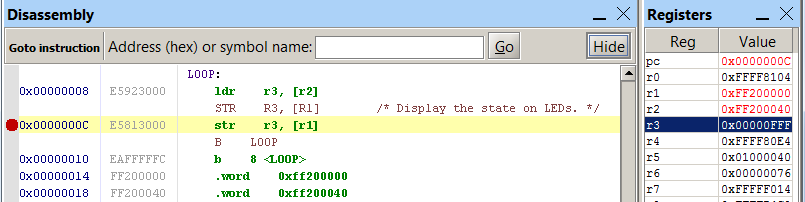
\includegraphics[scale=1]{screenshots/figure35.png}
   \end{center}
   \caption{Editing a register value.} 
   \label{fig:AMP_editregister_arm}
\end{figure}

\section{Using the Memory Window}

Clicking on the {\sf Memory} tab brings up the window in 
Figure \ref{fig:AMP_memorywindow}, which displays the contents
of the system's memory space and allows the user to edit memory
values. The leftmost column in the window gives a memory address,
and the numbers at the top of the window represent hexadecimal
address offsets from that corresponding address. 

\begin{figure}[H]
   \begin{center}
      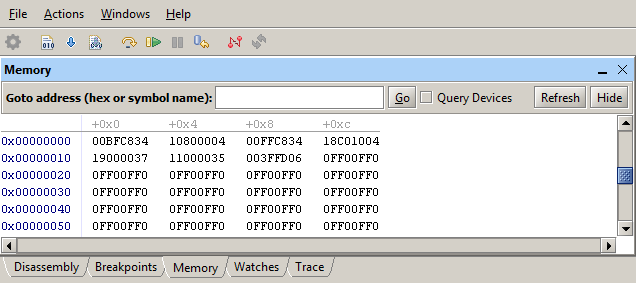
\includegraphics[scale=0.6]{screenshots/figure36.png}
   \end{center}
   \caption{The Memory window.} 
   \label{fig:AMP_memorywindow}
\end{figure}

\subsection{Examining and Changing Memory Contents}

If a program is running, the data values displayed in the
Memory window are not updated. But, when the program is stopped,
the data values are automatically updated. They can also be
updated by pressing the {\sf Refresh} button. 
By default, the Memory window shows only the contents of memory
devices, and does not display any values from memory-mapped I/O devices. To cause the window to display memory-mapped
I/O locations, click on the check mark beside 
{\sf Query Devices}, and then click 
{\sf Refresh}. For example, set the slider switches on the
DE1-SoC board to some pattern, press {\sf Refresh}, enter the
address \texttt{0xFF200040} and press {\sf Go}. 
Figure \ref{fig:AMP_memoryIO} shows the display we obtained when choosing the pattern
0x30F.

\begin{figure}[H]
   \begin{center}
      \includegraphics[scale=1]{screenshots/figure37.png}
   \end{center}
   \caption{Displaying the I/O locations.} 
   \label{fig:AMP_memoryIO}
\end{figure}

The color of a memory word displayed depends on whether that
location corresponds to an actual memory device, a memory-mapped
I/O device, or is not mapped at all in the system. 
A memory location that corresponds to a memory device will be 
colored black, as in Figure \ref{fig:AMP_memorywindow}. Memory-mapped I/O is shown in
blue color, and a non-mapped address is shown in grey. 
If a memory location changed value since it was previously
displayed, then that memory location is shown in a red color.

Similar to the Disassembly window, it is possible to view
different memory regions by scrolling using the vertical scroll
bar on the right, or by using a mouse scroll wheel.
There is also a \textsf{Goto address} panel, in which we typed
the address \texttt{FF200040} to reach the I/O device as
depicted in Figure \ref{fig:AMP_memoryIO}.
  
As an example of editing a memory value, go to address
\texttt{FF200000} which is the address of LEDs.
Double-click on the memory word at this address 
and type the data value FFF. Press \textsf{Enter} on
the computer keyboard, or click away from the memory word to
apply the edit. This should cause all LEDs to be turned on. 

When accessing an I/O device, some reads may be destructive.
Namely, after some register in the I/O interface is read, its
contents may no longer be valid. Therefore, it is not
appropriate to read all I/O registers when refreshing the
information in the Memory window. Instead, it is prudent to read
only the registers that are of specific interest. This can be
accomplished  by left-clicking on the address of interest and
then right-clicking to update the displayed contents. Several
consecutive addresses can be selected by clicking on the first
address and dragging across the other addresses.

\subsection{Configurability of the Memory Window}

The Memory window is configurable in a variety of ways:

\begin{itemize}
\item Memory element size - the display can format the memory
contents as bytes, half-words (2-bytes), or words (4-bytes).
This setting can be configured by right-clicking on the Memory
window, as illustrated in Figure \ref{fig:AMP_memorysettings_1}.

\begin{figure}[H]
   \begin{center}
      \includegraphics[scale=0.7]{screenshots/figure38.png}
   \end{center}
   \caption{Setting the memory element size.} 
   \label{fig:AMP_memorysettings_1}
\end{figure}

\item Number of words per line - the number of words per line can
be configured to make it easier to find memory addresses, as
depicted in Figure \ref{fig:AMP_memorysettings_2}.

\begin{figure}[H]
   \begin{center}
      \includegraphics[scale=0.7]{screenshots/figure39.png}
   \end{center}
   \caption{Setting the number of words per line.} 
   \label{fig:AMP_memorysettings_2}
\end{figure}

\item Number format - this is similar to the number format option in the Register window described in Section 9,
and can be configured by right-clicking on the Memory window.

\item Display order - the Memory window can display addresses
increasing from left-to-right or right-to-left. 

\end{itemize}


\subsection{Character Display}

The \textsf{Memory} window can also be configured to interpret
memory byte values as ASCII characters. 
This is useful if one wishes to examine character strings that 
are stored in the memory.
For this purpose it is convenient to view
the memory in bytes and characters simultaneously so that the
characters appear in the correct sequence. This can be
accomplished by clicking the {\sf Switch to character mode} menu
item, as illustrated in Figure \ref{fig:AMP_memorysettings_3}. A sample display in the
character mode is shown in Figure \ref{fig:AMP_memorycharactermode}.
  
\begin{figure}[H]
   \begin{center}
      \includegraphics[scale=0.7]{screenshots/figure40.png}
   \end{center}
   \caption{Switching to the character mode.}
   \label{fig:AMP_memorysettings_3}
\end{figure}

\begin{figure}[H]
   \begin{center}
      \includegraphics[scale=0.7]{screenshots/figure41.png}
   \end{center}
   \caption{Character mode display.}
   \label{fig:AMP_memorycharactermode}
\end{figure}

It is possible to return to the previous memory view mode by
right-clicking and selecting the {\sf Revert to previous mode}
menu item.


\subsection{Memory Fill}

Memory fills can be performed in the Memory window. Click the
{\sf Actions > Memory fill} menu item or right-click on the
Memory window and select {\sf Memory fill}. 
A {\sf Memory fill} panel will appear on the left side of the
Memory window, as shown Figure \ref{fig:AMP_memoryfill}. Fill in the desired values and 
click {\bf Fill}. A typical use of this may be to zero a range of memory locations.

\begin{figure}[H]
   \begin{center}
      \includegraphics[scale=0.7]{screenshots/figure42.png}
   \end{center}
   \caption{The Memory fill panel.} 
   \label{fig:AMP_memoryfill}
\end{figure}

\subsection{Save Memory Data to File}

The data that you see on the Memory window can be saved into a csv file 
on your computer. This feature is accessed by selecting the command 
{\sf Actions > Save memory onto disk} or by right-clicking on the
Memory window. The {\sf Save Memory} panel will appear on the left
side of the Memory window, as illustrated in Figure \ref{fig:AMP_memorysave}.
The user provides a filepath to save the generated file, a starting 
and ending address for the region of memory to save, and selects an
alignment for the memory to be saved as (ie. word-aligned means that
the memory will be saved one word at a time). 

Additionally, there is 
an option for whether or not to save header and address info. If this box
is checked, address numbers and offset headers for each chunk of memory
saved will be included in the csv file, allowing the user to determine
at which address each chunk of memory is stored. If this box is unchecked,
only the raw memory data will be saved into the csv file. This means that 
the user will have to keep track of which address region the saved file 
refers to, however, it also means that the saved csv file will be in the
correct format for use in the {\sf Load File Data into Memory} function in 
the Memory window.

Note that when you select to save a memory range, all memory addresses within
the range will be read, whether or not the read is destructive (ie. non-memory 
device addresses may also be read).

\begin{figure}[H]
	\begin{center}
		\includegraphics[scale=0.7]{screenshots/memory_save_window.png}
	\end{center}
	\caption{The Memory save panel.} 
	\label{fig:AMP_memorysave}
\end{figure}

\subsection{Load File Data into Memory}

Data stored in a file can be loaded into the memory by using the
Memory window. This feature is accessed by selecting the command
{\sf Actions > Load file into memory} or by right-clicking on the
Memory window. The {\sf Load file} panel will appear on the left
side of the Memory window, as illustrated in Figure \ref{fig:AMP_memoryload}, to allow
the user to browse and select a data file.  The user provides a base address in memory where the data should be stored. 

\begin{figure}[H]
   \begin{center}
      \includegraphics[scale=0.7]{screenshots/figure43.png}
   \end{center}
   \caption{The Load file panel.}
   \label{fig:AMP_memoryload}
\end{figure}

The format of these files is illustrated in Figure \ref{fig:example_delimited_hex_file}. 
The file consists of any number of lines, where each line
comprises a comma-separated list of data values. Each data value
is expressed as a hexadecimal number with an optional $-$ sign.
Two additional parameters can be specified: the value of the
delimiter character (comma is the default), and size in bytes of
each data value (1 is the default).

\begin{figure}[H]
   \begin{center}
      \includegraphics[scale=0.80]{screenshots/figure44.png}
   \end{center}
   \caption{A Delimited hexadecimal value file.}
   \label{fig:example_delimited_hex_file}
\end{figure}


\section{Working with Project Files}

Project files store the settings for a particular project, 
such as the specification of a hardware system and program source
files. A project file, which has the filename 
extension {\it .amp}, is stored into a project's directory when
the project is created. 

The Monitor Program provides the following commands, under the
{\sf File} menu, for working with project files:

\begin{enumerate}
    \item {\sf New Project}: Presents a series of screens that are used to create a new project.
    \item {\sf Open Project}: Displays a dialog to select an
existing project file and loads the project.
    \item {\sf Open Recent Project}:  Displays the five most recently used project files, and allows these projects to be
reopened.
    \item {\sf Save Project}: Saves the current project's
settings after they have been modified by using 
the {\sf Settings} command.
\end{enumerate}

\subsection{Modifying the Settings of an Existing Project}

After a project has been created, it is possible to modify many
of its settings, if needed. This can be done by clicking
on the menu item {\sf File > Edit Project} in the Monitor
Program. This action will display the existing system settings for the
project, and allow them to be changed. Note that to change
these settings, the Monitor Program has to first be disconnected
from the system being debugged. This can be done by using the
command {\sf Actions > Disconnect}, or by clicking the
\includegraphics{toolbar/disconnect.png} icon.

\newpage
\section{Using the Terminal Window}

Monitor Program's \emph{Terminal} window supports
text-based input and output. To see its operation, create
a new Monitor Program project, called {\it Monitor\_Terminal}.
When creating the project, follow the same steps shown for the
{\it Monitor\_Manual} project, which were illustrated in 
Section 3.1. For the screen shown in Figure \ref{fig:NPW_programtype} set the program
type to {\sf Assembly Program}, and in Figure \ref{fig:NPW_sampleprograms} select the
sample program named {\it JTAG UART}. The source code file for
that program is called {\it JTAG\_UART.s}.  It communicates using
memory-mapped I/O with the JTAG UART in the DE1-SoC Computer that
is selected as the {\sf Terminal device} in the screen of 
Figure \ref{fig:NPW_systemparameters}. 

The Terminal window supports a subset of the control character
commands used for a de facto standard terminal, called 
the {\it VT100}.
The supported commands are listed in Table 1.
In this table \texttt{<ESC>} represents the ASCII character 
with the code \texttt{0x1B}.

\begin{table}[H]
    \centering
    \begin{tabular}{|l|p{4in}|}
        \hline
        Character Sequence&Description\\
        \hline
        \hline
        \texttt{<ESC>[2J}&Erases everything in the Terminal window\\
        \hline
        \texttt{<ESC>[7h}&Enable line wrap mode\\
        \hline
        \texttt{<ESC>[7l}&Disable line wrap mode\\
        \hline
        \texttt{<ESC>[\emph{\#}A}&Move cursor up by \emph{\#} rows or by one row if \emph{\#} is not specified\\
        \hline
        \texttt{<ESC>[\emph{\#}B}&Move cursor down by \emph{\#} rows or by one row if \emph{\#} is not specified\\
        \hline
        \texttt{<ESC>[\emph{\#}C}&Move cursor right by \emph{\#} columns or by one column if \emph{\#} is not specified\\
        \hline
        \texttt{<ESC>[\emph{\#}D}&Move cursor left by \emph{\#} columns or by one column if \emph{\#} is not specified\\
        \hline
        \texttt{<ESC>[\emph{$\#_1$};\emph{$\#_2$}f}&Move the cursor to row \emph{$\#_1$} and column \emph{$\#_2$}\\
        \hline
        \texttt{<ESC>[H}&Move the cursor to the home position (row 0 and column 0)\\
        \hline
        \texttt{<ESC>[s}&Save the current cursor position\\
        \hline
        \texttt{<ESC>[u}&Restore the cursor to the previously saved position\\
        \hline
        \texttt{<ESC>[7}&Same as \texttt{<ESC>[s}\\
        \hline
        \texttt{<ESC>[8}&Same as \texttt{<ESC>[u}\\
        \hline
        \texttt{<ESC>[K}&Erase from current cursor position to the end of the line\\
        \hline
        \texttt{<ESC>[1K}&Erase from current cursor position to the start of the line\\
        \hline
        \texttt{<ESC>[2K}&Erase entire line\\
        \hline
        \texttt{<ESC>[J}&Erase from current line to the bottom of the screen\\
        \hline
        \texttt{<ESC>[2J}&Erase from current cursor position to the top of the screen\\
        \hline
        \texttt{<ESC>[6n}&Queries the cursor position. A reply is sent back in the format \texttt{<ESC>[\emph{$\#_1$};\emph{$\#_2$}R},
            corresponding to row \emph{$\#_1$} and column \emph{$\#_2$}.\\
        \hline
    \end{tabular}
    \caption{VT100 commands supported by the Terminal window.} 

\end{table}

\newpage
\subsection{The Nios II Terminal Example}
\label{tut:nios_6}

Compile, load and run the {\it JTAG\_UART.s} program.
Upon downloading the Nios II program, the Monitor Program
window should appear as shown in Figure \ref{fig:AMP_terminal_nios}. 
Click the mouse inside the Terminal window. Now, any characters
typed on the computer keyboard are sent by the Monitor Program to
the JTAG UART. These characters are shown in the Terminal window
as they are typed, because the {\it JTAG\_UART.s} program echoes
the characters back to the Terminal window.

{\it To continue to the next section of the Nios II tutorial, click \hyperref[tut:nios_7]{here}.}

\begin{figure}[H]
   \begin{center}
      \includegraphics[scale=0.6]{screenshots/figure45.png}
   \end{center}
   \caption{Using the Terminal window with a Nios II program.}
   \label{fig:AMP_terminal_nios}
\end{figure}

\subsection{The ARM Terminal Example}
\label{tut:arm_5}

Compile, load and run the {\it JTAG\_UART.s} program.
Upon downloading the ARM program, the Monitor Program
window should appear as shown in Figure \ref{fig:AMP_terminal_arm}. 
Click the mouse inside the Terminal window. Now, any characters
typed on the computer keyboard are sent by the Monitor Program to
the JTAG UART. These characters are shown in the Terminal window
as they are typed, because the {\it JTAG\_UART.s} program echoes
the characters back to the Terminal window.

{\it To continue to the next section of the ARM tutorial, click \hyperref[tut:arm_6]{here}.}

\begin{figure}[H]
   \begin{center}
      \includegraphics[scale=0.6]{screenshots/figure46.png}
   \end{center}
   \caption{Using the Terminal window with an ARM program.}
   \label{fig:AMP_terminal_arm}
\end{figure}

\newpage
\section{Using C Programs}

C programs are used with the Monitor Program in a similar way as
assembly-language programs. In the window depicted in Figure \ref{fig:NPW_programtype}
it is necessary to select {\sf C Program}.
To see an example of a C program,
create a new Monitor Program project and choose
the C sample program called {\it JTAG UART}.  
This program includes a C source file named {\it JTAG\_UART.c},
which has the same functionality as the assembly-language code
used in the previous example. 
Compile and run the program to observe its behavior.

\subsection{The Nios II C-Program Example}
\label{tut:nios_7}

Figure \ref{fig:NPW_programdetails_nios} shows the window in which the program details are
specified, as introduced in Figure \ref{fig:NPW_sourcefiles}.
The C code in the file {\it JTAG\_UART.c} uses memory-mapped 
I/O to communicate with the JTAG UART. 

Alternatively, it is possible to
use functions from the standard C library {\it stdio.h}, such as
{\it putchar}, {\it printf}, {\it getchar}, and {\it scanf} for
this purpose.  Using these library functions impacts the size of
the Nios~II executable code that is produced when the C program
is compiled, by about 30 to 64 KBytes, depending on
which functions are needed.  It is possible to minimize the size
of the code generated for this library by checking the box labeled {\sf Use small C library} in 
Figure \ref{fig:NPW_programdetails_nios}. When this option is used the
library has reduced functionality. 
Some limitations of the small C library include: 
no floating-point support in the output routines, 
such as {\it printf}, and no support for input routines, 
such as {\it scanf} and {\it getchar}.
~\\

\begin{figure}[H]
   \begin{center}
      \includegraphics[scale=1]{screenshots/figure47.png}
   \end{center}
   \caption{Program details for the sample C program for the Nios II Processor.} 
   \label{fig:NPW_programdetails_nios}
\end{figure}

In Figure \ref{fig:NPW_programdetails_nios} the option {\sf Emulate unimplemented instructions}
is checked. This option causes the C compiler to include code for
emulating any operations that are needed to execute the C program
but which are not supported by the processor. For example, the
Nios~II Economy version does not include a {\it multiply}
instruction, but the C program may need to perform this
operation. By checking this option, a multiply instruction 
will be implemented in software (by using addition and shift
operations).

{\it To continue to the next section of the Nios II tutorial, click \hyperref[tut:nios_8]{here}.}

\newpage
\subsection{The ARM C-Program Example}
\label{tut:arm_6}

Figure \ref{fig:NPW_programdetails_arm} shows the window in which the source files are
specified, as introduced in Figure \ref{fig:NPW_sourcefiles}.
The C code in the file {\it JTAG\_UART.c} uses memory-mapped 
I/O to communicate with the JTAG UART.
~\\~\\

\begin{figure}[H]
   \begin{center}
      \includegraphics[scale=1]{screenshots/figure48.png}
   \end{center}
   \caption{Source files for the sample C program for the ARM Processor.} 
   \label{fig:NPW_programdetails_arm}
\end{figure}


Alternatively, it is possible to
use functions from the standard C library {\it stdio.h}, such as
{\it printf} and {\it scanf}. In this case it is necessary to
use the {\it Semihosting} terminal option, which can be selected 
when specifying the system parameters. Instead of the JTAG\_UART,
choose {\sf Semihosting} in the dropdown menu for the
{\sf Terminal device}, as shown in Figure \ref{fig:NPW_semihosting_arm}.

\begin{figure}[H]
   \begin{center}
      \includegraphics[scale=1]{screenshots/figure49.png}
   \end{center}
   \caption{Choosing the semihosting option.} 
   \label{fig:NPW_semihosting_arm}
\end{figure}

\newpage
Semihosting is a mechanism by which a
program running on an ARM processor can request services from
the debugger (Monitor Program). When an ARM program is compiled
by the Monitor Program, special C libraries are used which have
been modified to use the semihosting mechanism.
All C library functions that communicate with a terminal, such as 
{\it printf} and {\it scanf}, will send/receive text to/from
the Monitor Program's semihosting terminal. In effect,
semihosting allows the host computer to provide input and
output facilities that a system implemented on a DE1-SoC board
does not have.
A sample program, called {\it Semihosting Example}, is available
when specifying C as the program type.

{\it To continue to the next section of the ARM tutorial, click \hyperref[tut:arm_7]{here}.}

\section{Source Level Debugging}
The Monitor program supports common source level debugging features such as step over, step into, 
step out, and visualizing variables. The source level debugging feature of the Monitor Program is
a beta feature in the current release. This feature can be enabled and disabled at any point by 
going to the {\sf Edit} menu and selecting {\sf Edit > Enable Source Level Debugging}, or 
{\sf Edit > Disable Source Level Debugging}, depending on whether the feature is currently disabled or enabled respectively.
Figure~\ref{fig:AMP_editor} shows the Monitor Program's text editor, which is enabled alongside 
the enabling of source level debugging. The editor will be disabled
during the debug session, and re-enabled when the debug session is exited. 

\subsection{Debugging and Optimization Levels} \label{sec:optimization_levels}
There are several settings that can affect the detail provided by the debugger feature.

Depending on the optimization level of the compiled program will affect the degree to which
variable view is available. Using an optimization level of 0 or 1 allows the Monitor Program to read and display 
variables during debugging. Additionally, when using optimization level 1, some variable values
may not be able to be viewed at certain PC values, and some variables that have been optimized out
may not be able to be viewed at all.

The optimization level for a C-Program project and be found by going to the project settings ({\sf File > Edit Project}) 
and navigating to the {\it Program Settings} tab. In the {\it Compiler Flags} input box, 
ensure that the optimization level is set to either 0 or 1, by replacing {\it -O, -O2, } 
or {\it -O3} flag with {\it -O0} or {\it -O1} to allow variable view. 

Another option for debugging detail is found under {\sf Edit > Enable Extended Debugging Info}.
Turning on this option tells the debugger to track more variable information during runtime,
which allows some variable values to be viewed at more PC values than before. However, the
tracking of extended debugging information also slows down the running speed of the program.
Depending on the program, the speed slowdown may vary.

Finally, note that currently, source level debugging for programs with interrupts is only supported
when compiling with optimization level 1 or higher.

\begin{figure}[h]
	\begin{center}
		\includegraphics[scale=0.5]{screenshots/AMP_editor.png}
	\end{center}
	\caption{The Monitor Program with a source file open in editor view.}
	\label{fig:AMP_editor}
\end{figure}

\subsection{Using Breakpoints}
Once a program is loaded, C source files that are part of the compiled program 
may be opened by navigating to the {\sf Editor} window of the Monitor Program and then
selecting {\sf File > Open...} or by navigating to the {\sf Project Files} window and
double clicking a file.

On a file opened in the editor pane,  breakpoints can be toggled on a line of source code by clicking on the numbers to the 
left of the source code text. If a breakpoint does not show up on the line similar to Figure~\ref{fig:AMP_editor_breakpoint}, the line of source code 
likely does not correspond to an instruction. If this happens, try choosing a different line.

Setting or removing a breakpoint on a source line is a macro for setting or removing breakpoints
at each assembly instruction that the source line corresponds to. After setting a breakpoint
at a source line, you can notice that corresponding breakpoints are set at the instruction level
in the disassembly window. In the Disassembly view the source level breakpoint is marked with a red 
square as in Figure~\ref{fig:AMP_editor_sourcebreakpoint}. This differentiates source level breakpoints from instruction level breakpoints.
Note that one line of source code may correspond to multiple, not necessarily contiguous, lines of assembly code.

\begin{figure}[h]
	\begin{center}
		\includegraphics[scale=0.4]{screenshots/AMP_editor_breakpoint.png}
	\end{center}
	\caption{Setting a breakpoint in the editor view.}
	\label{fig:AMP_editor_breakpoint}
\end{figure}

\begin{figure}[h]
	\begin{center}
		\includegraphics[scale=0.4]{screenshots/AMP_editor_breakpointhit.png}
	\end{center}
	\caption{Hitting a breakpoint in the editor view.}
	\label{fig:AMP_editor_breakpointhit}
\end{figure}

\begin{figure}[h]
	\begin{center}
		\includegraphics[scale=0.4]{screenshots/AMP_editor_sourcebreakpoint.png}
	\end{center}
	\caption{Source level breakpoint in the disassembly view.}
	\label{fig:AMP_editor_sourcebreakpoint}
\end{figure}

\subsubsection{Source Level Debugging Actions}

\begin{figure}[h]
	\begin{center}
		\includegraphics[scale=1]{screenshots/AMP_debugactionbuttons.png}
	\end{center}
	\caption{Step Over, Step Into, Step Out toolbar icons}
	\label{fig:AMP_debugactionbuttons}
\end{figure}
To enable access to many of the source level debugging actions, the execution of a loaded program must first
be stopped at a line of source code. One way this can be accomplished is by setting a breakpoint at a line of source code
and continuing execution ({\sf Actions > Continue} or by clicking the green arrow on the toolbar) until that point.
Once the program halts, the Monitor Program should look similar to Figure~\ref{fig:AMP_editor_breakpointhit}. 

A Step Into action can be performed by selecting {\sf Actions > Step Into}, or by using the main toolbar button shown in Figure \ref{fig:AMP_debugactionbuttons}.
This will step to the next line of source code to be executed. If the program steps into a function in another file, the Monitor
Program will open the file in a new tab and highlight the line.

A Step Out action can be performed by selecting {\sf Actions > Step Out}, or by using the main toolbar. This will step out of the current function 
by executing until the first line of source code after returning from the current function. The Monitor Program will print an error to the
{\sf Info \& Errors} window if it cannot step out of the current function. This may occur if the program is currently in the
{\it main} function, if the function is not user-written, or if the function does not return. 

The Step Over action ({\sf Actions > Step Over}) moves to the next line of source code without stepping into functions. 
Execution will continue to the next line of source code inside the current function, or the first line of source code
in the parent function if a return is hit before a new line of source code.

Note that each of these actions may not always visually appear to be performing the desired action (ie. step over may not always
visually step to the line of source code that is directly below the current line). This is usually due to optimizations that
the compiler makes to eliminate/rearrange source lines when translated into assembly. If a source level action appears to do
something weird, make sure to check what is really going on in the {\sf Disassembly} window.

\subsection{Variable Values}

\begin{figure}[h]
	\begin{center}
		\includegraphics[scale=0.7]{screenshots/AMP_variablevalues.png}
	\end{center}
	\caption{Monitor Program Variable View.}
	\label{fig:AMP_variablevalues}
\end{figure}

The \productNameMed's  {\sf Variables} view displays the value of C program variables when the program is halted, as seen in Figure \ref{fig:AMP_variablevalues}.
Some variable types such as Arrays,  Typedefs, Structures and Unions will be expandable in the view. Use the {\sf +} button to 
expand and view the variables contents. Right clicking on a variable presents the options to jump to the declaration of the variable,
and the display format of the variable.

{\sf Go To Declaration} will open the file the variable is declared in and scroll to the declaration line number.
{\it Display As...} will change the format in which the variable is displayed.

The availability of viewing variable values varies with the optimization level among several other factors. For more information, refer to
\hyperref[sec:optimization_levels]{Section \ref{sec:optimization_levels}.}

\subsection{Setting the Optimization Level in Programs with Driver Support.}
To set the optimization level for a {\it Program with Driver Support} (or BSP), first create a TCL script in the base directory of the project (the same directory as your AMP project file). The TCL file should have a {\it .tcl} file extension, for example {\it config.tcl}. Open this file in a text editor and add the single line:\\
{\bf set\_setting hal.make.bsp\_cflags\_optimization -O0}\\
Where the argument {\it -O0} above is the desired optimization level. Now open the project settings in the Monitor Program and navigate to the {\it Program Settings} tab. In the {\it BSP settings TCL script} input box (shown in Figure~\ref{fig:NPW_tclScript}) enter the path to the TCL script you just created, or use the {\it Browse} button to search for it.

\begin{figure}[H]
	\begin{center}
		\includegraphics[scale=0.6]{screenshots/tclScript.png}
	\end{center}
	\caption{Adding a TCL script to a Program with Driver Support.}
	\label{fig:NPW_tclScript}
\end{figure}

Click the {\it Finish} button to close the dialog and save and compile the project. The optimization level should be set for both the generated (BSP) files, as well as your project files.

\clearpage
\newpage
\section{Using the Monitor Program with Exceptions and Interrupts}

The Monitor Program supports the use of exceptions and interrupts
in programs. To enable the proper handling of exceptions and 
interrupts it is necessary to specify the memory settings as
required by a given processor. Figure \ref{fig:NPW_memoryoptions} indicates the memory 
settings if exceptions and interrupts are not used. For the 
Nios II and ARM processors it is necessary to set the memory
assignments differently, as explained in the examples below.

\subsection{Exceptions and Interrupts with the Nios II Processor}
\label{tut:nios_8}

The following discussion shows how interrupts can be used with
both assembly-language and C-language programs.

\subsubsection{Interrupts with Assembly-Language Programs}

To see an example using interrupts with assembly-language code, 
create a new Monitor Program project
called {\it Monitor\_Interrupts}. When creating the new project
set the program type to assembly language and select the sample
program named {\it Interrupt Example}. 
Figure \ref{fig:NPW_interrupts_sourcefiles_nios} lists the source files for this sample program. 
The main program for the example is the file 
{\it interrupt\_example.s}, which initializes some I/O devices
and enables Nios~II interrupts. The other source files provide
the reset and exception handling for the program, and two interrupt-service routines.

\begin{figure}[H]
   \begin{center}
      \includegraphics[scale=1]{screenshots/figure50.png}
   \end{center}
   \caption{The source files for the Nios II interrupt example.} 
   \label{fig:NPW_interrupts_sourcefiles_nios}
\end{figure}

 
Figure \ref{fig:NPW_interrupts_memorysettings_nios} shows the required memory settings for this program.
The reset vector of the Nios~II processor is at address 
\texttt{0x0} and the exceptions vector is at address 
\texttt{0x20}. Enough space has to be left between the exceptions
vector location and the text section of the program to
accommodate the exceptions-processing code,
which corresponds to the assembly-language code in the 
file {\it exception\_handler.s}. 
Starting the main program at address \texttt{0x200}, as shown
in the figure, leaves enough space to accommodate the exception
processing code for this example.

\begin{figure}[H]
   \begin{center}
      \includegraphics[scale=1]{screenshots/figure51.png}
   \end{center}
   \caption{Memory settings for the Nios II interrupt example.} 
   \label{fig:NPW_interrupts_memorysettings_nios}
\end{figure}

Compile and load the program. Then, scroll the Disassembly window
to the label {\it EXCEPTION\_HANDLER}, which is at
address \texttt{0x00000020}.  
As illustrated in Figure \ref{fig:AMP_interrupts_exceptionhandler_nios}, set a breakpoint at this address.
Run the program. When the breakpoint is reached, single step
the program a few more instructions to determine the cause of the
interrupt. The source of the interrupt is a circuit in the 
DE1-SoC Computer called the {\it interval timer}. This 
citcuit provides the ability to generate an interrupt whenever a
specified time period elapses. Single step the program until the
processor enters the interrupt-service routine for the interval
timer. This routine first clears the timer register that caused
the interrupt, so that an interrupt request will not be raised
immediately again, and then performs other functions needed for
the program.

\begin{figure}[H]
   \begin{center}
      \includegraphics[scale=0.6]{screenshots/figure52.png}
   \end{center}
   \caption{The exception handler.} 
   \label{fig:AMP_interrupts_exceptionhandler_nios}
\end{figure}

Finally, remove the breakpoint that was set earlier, at address
\texttt{0x00000020}, and then select the \textsf{Continue}
command to run the program. Observe that the program displays a
rotating pattern across the HEX displays on the DE1-SoC board.
The direction of rotation can be changed by pressing the
pushbuttons KEY$_1$ or KEY$_2$ on the DE1-SoC board, and the
pattern can be changed to correspond to the
values of the slider switches by pressing KEY$_3$.  
%Pressing KEY$_0$ causes a reset of the Nios~II
%processor and returns control to the Monitor Program at the
%address \texttt{0x0}.

\subsubsection{Interrupts with C Programs}

To see an example of a C program that uses interrupts, create a
new project called {\it Monitor\_Interrupts\_C}.
When creating this project, set the program type to 
{\sf C Program} and select the sample program named 
{\it Interrupt Example}; this program gives C code that performs
the same operations as the assembly-language code in the previous
example. The source files for this example are listed in 
Figure \ref{fig:NPW_interrupts_c_sourcefiles_nios}. The main program is given in the file 
{\it interrupt\_example.c}, and the other source files provide
the reset and exception handling for the C program, as well as
two interrupt-service routines.  Complete the steps for creating
the project, and then compile and load it.

Set a breakpoint at the address \texttt{0x00000020}, which is the
exception vector address for the Nios~II processor.  Also, scroll
the Disassembly window to the function called 
{\it interrupt\_handler}. As illustrated in Figure \ref{fig:AMP_interrupts_interrupthandler_nios}, set
another breakpoint at this address. Now, run the program to reach
the first breakpoint, at address \texttt{0x00000020}. 
The code at this address, which is found in the file
{\it exception\_handler.c}, reads the contents of a control
register in the Nios~II processor to determine if the interrupt
is caused by an external device, then saves registers on the
stack, and then calls the {\it interrupt\_handler} function.

\newpage
\begin{figure}[H]
   \begin{center}
      \includegraphics[scale=1]{screenshots/figure53.png}
   \end{center}
   \caption{The source files for the C-code interrupt example.} 
   \label{fig:NPW_interrupts_c_sourcefiles_nios}
\end{figure}

~\\
~\\
\begin{figure}[H]
   \begin{center}
      \includegraphics[scale=1]{screenshots/figure54.png}
   \end{center}
   \caption{The interrupt handler.} 
   \label{fig:AMP_interrupts_interrupthandler_nios}
\end{figure}


Press {\sf Actions > Continue} in the Monitor Program to reach
the second breakpoint. Single stepping the program a few more
instructions shows that the interrupt is caused by the interval
timer in the DE1-SoC Computer, as discussed in the previous
example. Additional single stepping causes the processor to enter
the interrupt-service routine for the interval timer,
as depicted in Figure \ref{fig:AMP_interrupts_isr_nios}. This routine first clears the timer
register that caused the interrupt, and then performs other
functions needed for the program.
Finally, clear both breakpoints that were set earlier, at address
\texttt{0x00000020} and {\it interrupt\_handler}, and then run
the program; it displays a rotating pattern on the HEX displays
of the DE1-SoC board, as discussed in the previous example.

{\it This is the end of the Nios II tutorial.}


\begin{figure}[H]
   \begin{center}
      \includegraphics[scale=1]{screenshots/figure55.png}
   \end{center}
   \caption{The interrupt service routine for the interval timer.} 
   \label{fig:AMP_interrupts_isr_nios}
\end{figure}


\subsection{Exceptions and Interrupts with the ARM Processor}
\label{tut:arm_7}

The discussion below shows how interrupts can be used with
both assembly-language and C-language programs. In an 
ARM-based system, interrupt requests are handled by the
Generic Interrupt Controller. Consult the tutorial
{\it Using the ARM Generic Interrupt Controller}, which is
available at the Intel website, for a description of how
interrupts are processed.

\subsubsection{Interrupts with Assembly-Language Programs}

To see an example using interrupts with assembly-language code, 
create a new Monitor Program project.
When creating the new project choose the ARM processor,
set the program type to assembly language and select the sample
program named {\it Interrupt Example}. 
Figure \ref{fig:NPW_interrupts_sourcefiles_arm} lists the source files for this example.
The main program is in the file {\it interrupt\_example.s}.
Comments given in this file explain the behavior of the program.

\begin{figure}[H]
   \begin{center}
      \includegraphics[scale=1]{screenshots/figure56.png}
   \end{center}
   \caption{The assembly-language source files for the ARM interrupt example.} 
   \label{fig:NPW_interrupts_sourcefiles_arm}   
\end{figure}

 
Figure \ref{fig:NPW_interrupts_memorysettings_arm} shows the required memory settings for this example.
The memory locations in the address range \texttt{0x0} to
to \texttt{0x3F} must be reserved for vectors used in various
exceptions and interrupts. The main program can start at
address \texttt{0x40}.

Complete the project, download the program and run it to observe
its behavior.   


\begin{figure}[H]
   \begin{center}
      \includegraphics[scale=0.6]{screenshots/figure57.png}
   \end{center}
   \caption{Memory Settings for the ARM interrupt example.} 
   \label{fig:NPW_interrupts_memorysettings_arm}
\end{figure}

\newpage
\subsubsection{Interrupts with C Programs}

To see an example using interrupts with C code, 
create a new Monitor Program project.
When creating the new project choose the ARM processor,
set the program type to C language and select the sample
program named {\it Interrupt Example}. 
Figure \ref{fig:NPW_interrupts_c_sourcefiles_arm} lists the source files for this example.
The main program is in the file {\it interrupt\_example.c}.
Comments given in this file explain the behavior of the program.
Complete the project, download the program and run it to
observe its behavior.

{\it This is the end of the ARM tutorial}

\begin{figure}[H]
   \begin{center}
      \includegraphics[scale=1]{screenshots/figure58.png}
   \end{center}
   \caption{The C-language source files for the ARM interrupt example.} 
   \label{fig:NPW_interrupts_c_sourcefiles_arm}
\end{figure}


\section{Working with Windows and Tabs}

It is possible to rearrange the Monitor Program workspace by
moving, resizing, or closing the internal windows inside the main
Monitor Program window.

To move a particular window to a different location, click on the
window title or the tab associated with the window, and drag the
mouse to the new location. As the mouse is moved across the main
window, the dragged window will snap to different locations. 
To detach the dragged window from the main window, drag it beyond
the boundaries of the main window. 
To re-attach a window to the main window, drag the tab associated
with the window onto the main window.

To resize a window, hover the mouse over one of its borders, and
then drag the mouse. Resizing a window that is attached to the
main window will cause any adjacent attached windows to also
change in size accordingly.

To hide or display a particular window, use the {\sf Windows}
menu. To revert to the default window arrangement, simply exit
and then restart the Monitor Program. Figure \ref{fig:AMP_rearrangedworkspace} shows an example
of a rearranged workspace.

\begin{figure}[H]
   \begin{center}
      \includegraphics[scale=0.6]{screenshots/figure59.png}
   \end{center}
   \caption{The \productNameMed{} with a rearranged workspace.} 
   \label{fig:AMP_rearrangedworkspace}
\end{figure}


\section{Using the Watches Window}

Watch expressions provide a convenient means of keeping track of
the value of multiple expressions of interest. These expressions
are re-evaluated each time program execution is stopped. 
To add a watch expression:

\begin{enumerate}
\item Switch to the {\it Watches} window.

\item Right-click on the gray bar and click \textsf{Add},
as illustrated in Figure \ref{fig:AMP_watches}.

\begin{figure}[H]
   \begin{center}
      \includegraphics[scale=1]{screenshots/figure60.png}
   \end{center}
   \caption{The Watches window.}
   \label{fig:AMP_watches}
\end{figure}

\item The {\it Edit Watch Expression} window will appear, as
shown in Figure \ref{fig:AMP_editwatchexpression}. The desired watch expression can then be
entered, using the syntax indicated in the window. In the figure,
the expression \texttt{mem32(sp)} is entered, which will display
the value of the data word at the current stack pointer address.

\begin{figure}[H]
   \begin{center}
      \includegraphics[scale=1]{screenshots/figure61.png}
   \end{center}
   \caption{The Edit Watch Expression window.}
   \label{fig:AMP_editwatchexpression}
\end{figure}

\item Click \textsf{Ok}. The watch expression and its current
value will appear in the table. The number format of a value
displayed in the watch expression window can be changed by
right-clicking on the row for that value.  
As the program being debugged is repeatedly run, 
the watch expression will be re-evaluated each time and its value
will be shown in the table of watch values.
\end{enumerate}


\section{The GDB Server Panel (Advanced)}
To see this panel, select the {\sf GDB Server} panel of the
Monitor Program. This window will display the low-level commands
being sent to the GDB Server, used to interact with the HPS
system on the DE1-SoC board. It will also show the responses that GDB sends back. The Monitor Program provides the option
of typing GDB commands and sending them to the debugger. 
Consult online resources for the GDB program to learn what
commands are available.

\newpage
\section{Using Device Drivers (Advanced)}
Intel's development environment for Nios~II programs provides a
facility for using device driver functions for the I/O devices in
a hardware system. This facility, which is called the
{\it hardware abstraction layer} (HAL), is supported by the
Monitor Program. Using device driver functions is not recommended
for beginning students, and is intended for more advanced users. 

To see an example of code that uses device driver functions
create a project called {\it Monitor\_HAL}. 
Select the DE1-SoC Computer system. Set the program type to 
{\sf Program with Device Driver Support}, 
check {\sf Include a sample program with the project}, 
and select the sample program named {\it Media}. The source file
for this sample program is called {\it media.c}.
When creating this project, the New Project Wizard does not
display the screen for choosing memory settings, such as the one in Figure \ref{fig:NPW_interrupts_memorysettings_nios}. This is because the HAL automatically chooses 
the necessary memory settings for projects that make use of device drivers.

The {\it media.c} program communicates with I/O devices by making
calls to device driver functions, rather than using memory-mapped
I/O as has been done in previous examples in this document.  
To see some examples of such function-calls, examine the source
code in the file {\it media.c}. It calls device driver functions
for the audio devices in the DE1-SoC Computer, the VGA output
port, the PS/2 port, and parallel ports. The device driver
functions for each of these devices are defined in 
{\it include files} that are specified at the top of the
{\it media.c} file. The set of device driver functions
provided for an IP core is specified as part of the documentation
for that IP core.

Compile and load the program by using the command 
{\sf Actions > Compile \& Load}. 
The Monitor Program automatically compiles both the {\it media.c}
program and all device drivers that it uses. In subsequent
compilations of the program, only the {\it media.c} code is
compiled. 

Run the program. It performs the following: 
\begin{itemize}
\item
Records audio for about 10 seconds when KEY[1] is pressed. 
LEDR[0] is lit while recording.
\item 
Plays the recorded audio when KEY[2] is pressed. LEDR[1] is lit while playing.
\item
Draws a blue box on the VGA display, and places a text string inside the box.
\item
Shows on the HEX displays the last three bytes of data received from a device connected to the PS/2 port. 
\end{itemize}

More details about developing programs with the Monitor Program
that use HAL device drivers can be found in the tutorial 
{\it Using HAL Device Drivers with the \productNameMed{}}, which is available in the University Program section of Intel's
website. More information about HAL can be found in the
{\it Nios~II Software Developer's Handbook}.

\newpage
\section{Running Multiple Instances of the Monitor Program (Advanced)}

In some cases it may be useful to run more than one instance of
the Monitor Program on the same computer. For example, the
selected system may contain more than one processor. 
An instance of the Monitor Program is required to run and debug
programs on each available processor. As described in 
Section 3, it is possible to select a particular processor
in a system via the \textsf{Processor} drop-down
list in the {\it New Project Wizard} and {\it Project Settings}
windows.

The Monitor Program uses the {\it GDB Server} to interact with
the HPS system, and connects to the GDB Server using TCP ports.
By default, the Monitor Program uses port 2399 as the base port,
and to connect to each processor in a system the Monitor Program
will attempt to use a port located at a fixed offset from this
base port. For example, a single system consisting of four
processors corresponds to ports 2399-2402.

However, the Monitor Program does not detect any ports that may
already be in use by other applications. If the Monitor Program
fails to connect to the GDB Server due to a port conflict, then
the base port number can be changed by creating an environment
variable called \texttt{ALTERA\_MONITOR\_DEBUGGER\_BASE\_PORT}
and specifying a different number.

It is also possible to have more than one board connected to
the host computer. As described in Section 3.1, a particular
board can be selected via the \textsf{Host connection} drop-down
list in the {\it New Project Wizard} and {\it Project Settings}
windows. In this case, a separate instance of the Monitor
Program is needed to interact with each processor on each
physical board. By default, the Monitor Program assumes a
maximum of ten Nios~II processors per board. This means that
ports 2399-2408 are used by the Monitor Program for the first
board connected to the computer, and the first processor on the
second board will use port 2409.

It is possible to specify a different value for the maximum
number of processors per Nios~II hardware system by creating an
environment variable called 
\texttt{ALTERA\_MONITOR\_DEBUGGER\_MAX\_PORTS\_PER\_CABLE} and
specifying a different number. 
This is useful if a system contains more than ten Nios~II
processors. It is also useful if a port conflict exists and none
of the systems contain ten or more processors. In this case,
decreasing this number (in conjunction with changing the base
port number) may provide a solution.

\newpage
\section{Examining the Instruction Trace (Advanced)}

An instruction trace is a hardware-level mechanism to record a
log of all recently executed instructions. 
The \emph{Nios~II JTAG Debug Module} has the instruction trace
capability, but only if a Level 3 or higher debugging level
is selected in the \emph{SOPC Builder} or \emph{Platform Designer}
configuration of the JTAG Debug Module 
(See the \emph{Nios~II Processor Reference Handbook},
available from Intel, for more information about the
configuration settings of the JTAG Debug Module). If the 
required JTAG Debug Module is not present, a message will be
shown in the \textsf{Info \& Errors} window of the Monitor
Program after loading a program, to indicate that instruction
trace is not available.

The {\it Trace} feature is automatically enabled if the 
required JTAG Debug Module is available. To view the 
instruction trace of a program, go to the Trace window
after pausing the program during execution. As shown in 
Figure \ref{fig:AMP_traces}, the instructions are grouped into
different colored blocks and labeled alphabetically. 
The number of times each instruction block is executed is
shown beneath its alphabetical label.

\begin{figure}[H]
   \begin{center}
      \includegraphics[scale=1]{screenshots/figure62.png}
   \end{center}
   \caption{The Trace window.}
   \label{fig:AMP_traces}
\end{figure}

Right-clicking anywhere in the Trace window brings up
several options, as shown in Figure \ref{fig:AMP_trace_rightclick}.
The Trace feature can be turned on or off by selecting
the \textsf{Enable trace} or \textsf{Disable trace} options. 
It is also possible to toggle the {\it debug events} in the 
trace on or off by selecting \textsf{Show debug events}, or
clear current trace sequences by selecting 
\textsf{Clear trace sequences}. 

\begin{figure}[H]
   \begin{center}
      \includegraphics[scale=1]{screenshots/figure63.png}
   \end{center}
   \caption{Right-click options in the Trace window.}
   \label{fig:AMP_trace_rightclick}
\end{figure}

Running the program using the \textsf{Actions > Continue} or
\textsf{Actions > Single Step} commands will show up in the
trace sequence as {\it debug events} after each time the
program pauses execution, as shown in 
Figure \ref{fig:AMP_trace_debugevents}.

\begin{figure}[H]
   \begin{center}
      \includegraphics[scale=1]{screenshots/figure64.png}
   \end{center}
   \caption{The Trace window with various debug events.}
   \label{fig:AMP_trace_debugevents}
\end{figure}

If the {\it pc} value is changed before the program continues 
to run, the Monitor Program will insert a gap sequence in the
trace, as shown in Figure \ref{fig:AMP_trace_gap}. 
The \textsf{Actions > Restart} command will set the {\it pc}
value back to the initial starting address. The {\it pc} 
value can also be arbitrarily set by double clicking its value 
in the \textsf{Registers} window and editing
its hexadecimal value. 

\begin{figure}[H]
   \begin{center}
      \includegraphics[scale=1]{screenshots/figure65.png}
   \end{center}
   \caption{A gap sequence in the instruction trace.}
   \label{fig:AMP_trace_gap}
\end{figure}

Breakpoints in the program will also show up in the trace
sequence as a {\it debug event} each time the breakpoint
condition is met, as illustrated in Figure \ref{fig:AMP_trace_breakpoint}.

\begin{figure}[H]
   \begin{center}
      \includegraphics[scale=1]{screenshots/figure66.png}
   \end{center}
   \caption{A breakpoint in the instruction trace.}
   \label{fig:AMP_trace_breakpoint}
\end{figure} 

\subsection{Note About Tracing Interrupt Sequences}
It is possible that interrupt sequences are happening in the
program, yet do not show up in the Trace window in 
the Monitor Program. This is because the instruction blocks
shown in the trace sequence are actually sampled from a window 
of time over the entire program execution. As a result, the
interrupt sequences may not be included in the sample of
instruction blocks displayed in the Monitor Program. 
One way to deal with this problem is to trigger a breakpoint
after an interrupt finishes executing.

\section{Using the Monitor Program with a Nios~II Evaluation License}

In our discussion of Figure \ref{fig:NPW_downloadprompt} in Section 4,
we showed how the Monitor Program can be used to download a
prebuilt Nios~II hardware system onto an FPGA board, when the
Nios~II processor has a license. It is also possible to use the
Monitor Program to debug hardware systems in which the Nios~II
processor includes only an evaluation license. In this case
it is necessary to download the hardware system onto the FPGA
board by using the {\it Programmer} tool provided in the 
Quartus Prime software, rather than using the Monitor Program for
this purpose. The Quartus Prime Programmer tool provides a pop-up
window, shown in Figure \ref{fig:QUARTUS_programmerpopup}, which indicates activation of
the evaluation license for the Nios~II processor. 
This pop-up window has to remain open in order to maintain the
evaluation license for Nios~II. As long as the pop-up
window remains open, the Monitor Program can be used to compile
and download software programs into the hardware system.

\begin{figure}[H]
   \begin{center}
      \includegraphics[scale=1]{screenshots/figure67.png}
   \end{center}
   \caption{The Quartus Prime Programmer pop-up window.} 
   \label{fig:QUARTUS_programmerpopup}
\end{figure}


%%%%%%%%%%%%%%%%%%%%%%%%%%%%%%%%%%%
%%% Altera Copyright Information
%\newcommand{\datePublished}{Mar 2022}

\newcommand{\versnum}{21.1} %version number quartus/AMP
\newcommand{\quartusname}{Quartus\textsuperscript{\textregistered} Prime}	
\newcommand{\textBar}{For \quartusname{} \versnum{}}
\newcommand{\thisyear}{2022 } %for copyright
\newcommand{\company}{FPGAcademy.org}
\newcommand{\longteamname}{FPGAcademy.org}
\newcommand{\teamname}{FPGAcademy}
\newcommand{\website}{FPGAcademy.org}

\newcommand{\productAcronym}{AMP}
\newcommand{\productNameShort}{Monitor Program}

\newcommand{\productNameMedTM}{Monitor Program}
\newcommand{\productNameMed}{Monitor Program}

%\newcommand{\headerLogoFilePath}[1]{#1/FPGAcademy.png}



%%%%%%%%%%%%%%%%%%%%%%%%%%%%%%%%%%%%%%%%
%%% FPGAcademy Copyright Information %%%
%%%%%%%%%%%%%%%%%%%%%%%%%%%%%%%%%%%%%%%%

%Always put the copyright on a new page (clear page), with some vertical space from top
\clearpage
\vspace{1in}

\noindent

Copyright {\copyright} FPGAcademy.org. All rights reserved. FPGAcademy and the FPGAcademy logo are trademarks of  FPGAcademy.org.  This document is being provided on an ``as-is'' basis and as an accommodation and therefore all warranties, representations or guarantees of any kind (whether express, implied or statutory) including, without limitation, warranties of merchantability, non-infringement, or fitness for a particular purpose, are specifically disclaimed.

%FPGAcademy assumes no responsibility or liability arising out of the application or use of any information,  product,  or  service  described  herein  except  as  expressly  agreed  to  in  writing  by  FPGAcademy.



**Other names and brands may be claimed as the property of others.




\end{document}


